\documentclass[12pt]{book}

\usepackage[a4paper, 
    top=24mm, 
    bottom=24mm, 
    inner=32mm, 
    outer=25mm,
    marginparwidth=20mm,
    marginparsep=3mm,]{geometry}
\usepackage{graphicx}
\usepackage{wrapfig}
\usepackage{hyperref}
\usepackage{url}
\usepackage{listings}
\usepackage[dvipsnames]{xcolor}
\usepackage{minitoc}
\usepackage{comment}
\usepackage{lmodern}
\usepackage{anyfontsize}
\usepackage[italian]{babel}
\usepackage{amsmath,amssymb,amsfonts}
\usepackage{relsize}
\usepackage{xspace}
\usepackage{booktabs}
\usepackage{mathtools}
\usepackage{enumitem}
\usepackage{framed}
\usepackage{amsthm}
\usepackage{thmtools}
\usepackage{etoolbox}
\usepackage{fancybox}
\usepackage{fancyvrb}
\usepackage{marginnote}
\usepackage{eso-pic}
\usepackage{anyfontsize}
\usepackage{transparent}
\usepackage{mdframed}
\usepackage{needspace}
\usepackage{nicematrix}

\usepackage{tikz}
\usepackage{pgfplots}
\pgfplotsset{compat=1.17}
\usepackage{tkz-euclide}
\usetikzlibrary{calc}
\usetikzlibrary{matrix}
\usetikzlibrary{shapes, arrows}

\usepackage{color}
\usepackage{multicol}
\usepackage[most]{tcolorbox}
\usepackage{varwidth}

\usepackage{fancyhdr}
\usepackage[style=iso]{datetime2}

% \usepackage{charter}

\renewcommand*{\ttdefault}{qcr}


\lstset{
     literate=%
         {á}{{\'a}}1
         {à}{{\`a}}1
         {é}{{\'e}}1
         {è}{{\`e}}1
         {È}{{\`E}}1
         {…}{{\dots}}1
         {ù}{{\`u}}1
         {ò}{{\`o}}1
}

\newcommand{\Clang}[0]{C\xspace}
\newcommand{\matindex}[1]{\color{red}\tiny#1}

\usepackage{silence}

\WarningFilter{minitoc(hints)}{W0023}
\WarningFilter{minitoc(hints)}{W0028}
\WarningFilter{minitoc(hints)}{W0030}
\WarningFilter{minitoc(hints)}{W0024}


\newenvironment{myleftbar}{%
\def\FrameCommand{\hspace{0.6em}\textcolor{NavyBlue}{\vrule width 2pt}\hspace{0.6em}}%
\MakeFramed{\advance\hsize-\width \FrameRestore}\noindent\hspace{-0.5em}}%
{\endMakeFramed}


\declaretheoremstyle[
spaceabove=6pt,
spacebelow=1pt
headfont=\normalfont\bfseries,
headpunct={},
headformat={\cornersize*{2pt}\ovalbox{\NAME~{\color{NavyBlue}\NUMBER}}},
bodyfont=\normalfont,
]{exobreak}

\declaretheorem[parent=subsection, numberwithin=chapter, style=exobreak, name=Esercizio,%
postheadhook=\leavevmode\myleftbar,%
prefoothook =\endmyleftbar]{exercise}

\AtBeginEnvironment{exercise}{\Needspace{5\baselineskip}}

\newenvironment{solution}[2][]{
\vskip 1ex
\noindent\textbf{Soluzione all'esercizio~\ref{#2}}
#1
\vskip 1ex
}{}

\AtBeginEnvironment{solution}{\Needspace{5\baselineskip}}


\newcommand{\chapsubtitle}[1]{
\vspace{-1cm}
{\LARGE #1}
\vspace{1cm}
}

\newcommand{\exnote}[1]{%
\vspace{0.5em}%
\noindent\textbf{#1:}\xspace}

\lstdefinestyle{bashstyle}{%
language=Bash,
basicstyle=\footnotesize\ttfamily\color{white},%font size/family/etc. for source (e.g. basicstyle=\ttfamily\small)
backgroundcolor=\color{black},%colour for the background. External color or xcolor package needed.
commentstyle=\itshape\color{white},%style of comments in source language.
keywordstyle=\bfseries\color{white},%style of keywords in source language (e.g. keywordstyle=\color{red})
identifierstyle=\color{white},
emphstyle=\color{white},
stringstyle=\color{white},%style of strings in source language
showspaces=false,%emphasize spaces in code (true/false)
showtabs=false,%emphasize tabulators in code (true/false)
rulecolor=\color{black},
rulesepcolor=\color{black}
}

\lstdefinestyle{Rstyle}{%
language=R,
basicstyle=\footnotesize\ttfamily\color{black},%font size/family/etc. for source (e.g. basicstyle=\ttfamily\small)
backgroundcolor=\color{gray!10},%colour for the background. External color or xcolor package needed.
commentstyle=\itshape\color{gray!90},%style of comments in source language.
keywordstyle=\bfseries\color{NavyBlue},%style of keywords in source language (e.g. keywordstyle=\color{red})
identifierstyle=\color{NavyBlue},
emphstyle=\color{black},
stringstyle=\color{PineGreen},%style of strings in source language
showspaces=false,%emphasize spaces in code (true/false)
showstringspaces=false,% underline spaces within strings only
showtabs=false,%emphasize tabulators in code (true/false)
breaklines=true, % sets automatic line breaking
frame=single,% frame around code
rulecolor=\color{black},
rulesepcolor=\color{white},
keepspaces=true% keeps spaces in text, useful for keeping indentation of code (possibly needs columns=flexible)
}

\lstdefinestyle{Rstylescript}{%
language=R,
basicstyle=\footnotesize\ttfamily\color{black},%font size/family/etc. for source (e.g. basicstyle=\ttfamily\small)
backgroundcolor=\color{white},%colour for the background. External color or xcolor package needed.
commentstyle=\itshape\color{gray!90},%style of comments in source language.
keywordstyle=\bfseries\color{NavyBlue},%style of keywords in source language (e.g. keywordstyle=\color{red})
identifierstyle=\color{NavyBlue},
emphstyle=\color{black},
stringstyle=\color{PineGreen},%style of strings in source language
showspaces=false,%emphasize spaces in code (true/false)
showstringspaces=false,% underline spaces within strings only
showtabs=false,%emphasize tabulators in code (true/false)
breaklines=true, % sets automatic line breaking
frame=single,% frame around code
rulecolor=\color{black},
rulesepcolor=\color{white},
keepspaces=true% keeps spaces in text, useful for keeping indentation of code (possibly needs columns=flexible)
}


\lstdefinestyle{Rinlinestyle}{
    belowcaptionskip=1\baselineskip,
    breaklines=true,
    numbers=none,
    basicstyle=\ttfamily\small,
    keywordstyle=\bfseries\color{NavyBlue},
    commentstyle=\itshape\color{gray!90},
    identifierstyle=\bfseries\color{NavyBlue},
    stringstyle=\color{PineGreen},
    backgroundcolor=\color{gray!5!white},
    frame=single,
    rulecolor=\color{gray!50!white},
    showstringspaces=false,
}

\lstset{escapeinside={(*@}{@*)}}

\newcommand*\lsin{\lstinline[style=Rinlinestyle]}

\newtcolorbox{mybox}[2][]{empty, 
colframe=black, colback=gray!15, coltitle=black,
fonttitle=\bfseries\sffamily,
attach boxed title to top left={yshift=-2.5mm},
boxed title style={empty, size=small, top=1mm, bottom=0pt},
varwidth boxed title=0.5\linewidth,
frame code={
\path (title.east|-frame.north) coordinate (aux);
\path[draw=black, line width=0.5mm, rounded corners]
(frame.west) |- ([xshift=-2.5mm]title.north east) to[out=0, in=180] ([xshift=7.5mm]aux)-|(frame.east)|-(frame.south)-|cycle;  
},
title={#2},#1}

\lstset{
    style=bashstyle,
    language={bash}
}

% \lstset{
%     style=cppstyle,
%     language={C++}
% }

\lstset{
	style=Rstyle,
	language={R}
}  



\hypersetup{
    colorlinks=true,
    linkcolor=Brown,
    filecolor=magenta,
    urlcolor=MidnightBlue,
    pdftitle={Dispense C++},
    citecolor=ForestGreen,
    pdfpagemode=FullScreen,
}


\newenvironment{myitemize}
{ \begin{itemize}
    \setlength{\itemsep}{0pt}
    \setlength{\parskip}{0pt}
    \setlength{\parsep}{0pt}     }
{ \end{itemize}                  } 


\newenvironment{myenumerate}
{ \begin{enumerate}
    \setlength{\itemsep}{0pt}
    \setlength{\parskip}{0pt}
    \setlength{\parsep}{0pt}     }
{ \end{enumerate}  }


\tikzstyle{startstop} = [rectangle, rounded corners, minimum width=3cm, minimum height=1cm,text centered, draw=black]
\tikzstyle{code} = [rectangle, draw=none]
\tikzstyle{terminator} = [rectangle, draw, text centered, rounded corners, minimum height=2em]
\tikzstyle{process} = [rectangle, draw, text centered, minimum height=2em]
\tikzstyle{comment} = [rectangle, draw, text centered, minimum height=2em, text width=10em, fill=gray!20]
\tikzstyle{decision} = [diamond, draw, text centered, minimum height=2em, aspect=2]
\tikzstyle{data}=[trapezium, draw, text centered, trapezium left angle=60, trapezium right angle=120, minimum height=2em]
\tikzstyle{connector} = [draw, -latex']
\tikzstyle{commconn} = [draw, -latex',dashed]



\begin{document}

% \fancyhf{}
% % \fancyhead[RE,LO]{}
% \fancyfoot[RE,LO]{Autore: Alessia Visconti -- Versione: \today}
% \pagestyle{fancy}
%

\dominitoc


% \thispagestyle{empty}

% \AddToShipoutPictureBG*{\transparent{0.3}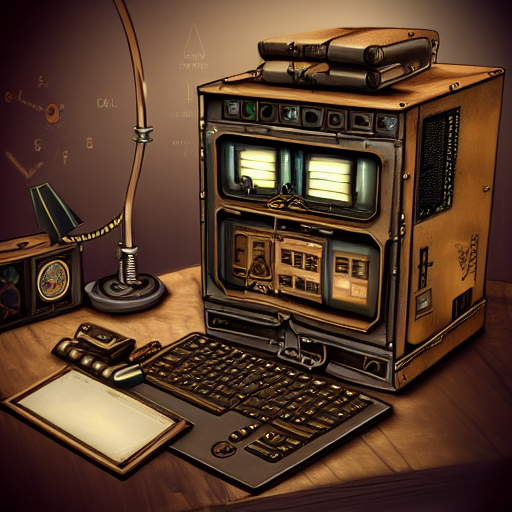
\includegraphics[width=2.4\columnwidth]{images/cover}}

\ 
\vspace{-2cm}
\begin{center}
{\sffamily\fontsize{20pt}{24pt}\selectfont \textbf{Alessia Visconti}\\}
\vspace{2cm}
{\sffamily\fontsize{40pt}{44pt}\selectfont \textbf{Introduzione all'analisi statistica dei dati in R}\\}
% \vspace{2cm}
% {\sffamily\fontsize{32pt}{40pt}\selectfont \textbf{Diario delle lezioni per il corso di Informatica per il CdL in Matematica}\\}
\vspace{2cm}
{\sffamily\fontsize{12pt}{14pt}\selectfont \textbf{Versione: \today}\\}
\vspace{8cm}

\includegraphics[width=0.25\columnwidth]{images/logo-unito.png}
\end{center}



\pagebreak


\tableofcontents

\chapter{Presentazione del Corso}


\section{Argomenti trattati}
\label{sec:presentazione}

Queste dispense si basano (Capitoli~\ref{cap:installareR}~-~\ref{cap:dati}), sul corso \textbf{R for Reproducible Scientific Analysis}, sviluppato dal collettivo \textbf{Software Carpentries}. Per motivi di tempo, ci concentreremo solo sulle funzioni che permettono semplici manipolazioni e analisi dei dati. 

\noindent I Capitoli~\ref{cap:descrittiva} e~\ref{cap:inferenziale} rappresentano del materiale originale, sviluppato appositamente per questo corso dal docente (Alessia Visconti, \href{mailto:alessia.visconti@unito.it}{alessia.visconti@unito.it}) e sono legati agli argomenti introdotti in modo teorico nella prima parte del corso di Statistica Medica. 

\noindent Non affronteremo nessun elemento di programmazione in R, che \`e al di fuori dello scopo di questo corso e neppure concetti avanzati di statistica. Per approfondimenti si rimanda alla Sezione~\ref{sec:corsi_carpentries}. 


% \secton{Perch\'e fare un laboratorio di R?}
%
% FIXME

\section{Approfondimenti}
\label{sec:corsi_carpentries}

Per chi volesse approfondire gli argomenti trattati, si rimanda al corso citato in Sezione~\ref{sec:presentazione}, ma anche al principale corso in programmazione R sviluppato dalle Carpentries, elencati in seguito. Entrambi i corsi sono pensati per persone che non hanno alcuna esperienza con la programmazione e/o l'analisi dati e alcuni argomenti sono ripetuti tra i due corsi:

\begin{myitemize}
	\item R for Reproducible Scientific Analysis \\ \url{https://swcarpentry.github.io/r-novice-gapminder}
	\item Programming with R \\ \url{https://swcarpentry.github.io/r-novice-inflammation}
\end{myitemize}

\noindent Esistono anche corsi in R specifici per alcune discipline, sempre sviluppati dalle Carpentries, che potete trovare al seguente indirizzo: \url{https://datacarpentry.org/lessons/}, insieme a molti altri corsi.

\noindent Se vi appassionate all'argomento, vi consiglio anche i seguenti testi, tutti disponibili gratuitamente online agli indirizzi indicati: 

\begin{myitemize}
	\item \textbf{R for Data Science} \\ \url{https://r4ds.had.co.nz/}
	\item \textbf{Learning Statistics with R}\footnote{L'autrice di questo libro, Danielle Navarro, si occupa anche di Generative Art e ha un blog molto interessante su R e Data Science. Trovate altro materiale che ha sviluppato nel suo sito: \url{https://djnavarro.net/}} \\ \url{https://learningstatisticswithr.com/lsr-0.6.pdf}
	\item \textbf{ggplot2: Elegant Graphics for Data Analysis} \\ \url{https://ggplot2-book.org/}
\end{myitemize}
	
\section{Ringraziamenti}

Vorrei ringraziare le Carpentries, non solo per il materiale che forniscono gratuitamente, ma anche per avermi reso un docente migliore, sotto molti punti fui vista. Ringrazio anche il professor Roberto Esposito, per avermi permesso di utilizzare il template \LaTeX ~che ha ideato -- le variazioni che lo rendono meno accattivante graficamente sono tutte mie. 


\noindent Per ultimo, un grosso grazie agli studenti del corso di laurea in Tecniche della Riabilitazione Psichiatrica, a.a. 2024/25, per essere stati i beta-tester di questo corso.


\section{Licenza}


This work is licensed under a Creative Commons Attribution-NonCommercial-ShareAlike 4.0 International License (cc-by-nc-sa).
See \url{http://creativecommons.org/licenses/by-nc-sa/4.0/} for details. 

\vspace{0.5cm}

\begin{figure}[h!]
 \centering
  
\includegraphics[width=0.25\textwidth]{images/CC BY-NC-SA 4.0.png}
\end{figure}
\chapter{Prepariamoci a partire...}
\label{cap:installareR}

% Circa 30m

\section*{Obiettivi di apprendimento}


\begin{multicols}{2}
\begin{tcolorbox}[width=1\linewidth, halign=left, colframe=blue!60, colback=white, boxsep=1mm, arc=3mm]

Domande

\begin{myitemize}
	\item Cos'\`e R?
	\item Cos'\`e RStudio?
	\item Come vengono installati?
	\item Che dati useremo in questo corso?
\end{myitemize}

\end{tcolorbox} 
\columnbreak
\begin{tcolorbox}[width=1\linewidth, halign=left, colframe=blue!60, colback=white, boxsep=1mm, arc=3mm]

Obiettivi

\begin{myitemize}
	\item Installare R e RStudio
\end{myitemize}

\end{tcolorbox} 
\columnbreak
\end{multicols}





\section{Il linguaggio di programmazione R}
\label{sec:Rintro}

R è un linguaggio di programmazione che è particolarmente utile e versatile per l'esplorazione, visualizzazione e analisi statistica dei dati. 

\noindent La sua versatilit\`a, il fatto che sia OpenSource e gratuito, la disponibilit\`a di una documentazione solida e di una vibrante comunit\`a e la possibilit\`a di estenderne le funzionalit\`a attraverso numerosi pacchetti lo hanno reso uno dei linguaggi pi\`u usati in numerosi campi, tra cui la ricerca biomedica, sopratutto la bioinformatica, l'epidemiologia, il data mining, l'econometria e la finanza, solo per citarne alcuni. 

 

\section{L'IDE RStudio}
\label{sec:RStudiointro}

R viene installato con un'interfaccia a linea di comando, ma \`e compatibile con diverse integrated development environment (IDE). Una IDE è un'applicazione  a software che aiuta i programmatori, ma anche gli analisti, a sviluppare codice e a interagire con i dati in modo semplice ed efficiente.

\noindent Per interagire con R utilizzeremo RStudio, che \`e una delle interfacce pi\'u usate.



\section{Perch\'e usare R?}

In questa parte del corso andremo a vedere gli aspetti basilari di R per l'esplorazione dei dati e la loro analisi statistica. 

\noindent Molto (se non tutto) quello che vedremo pu\`o anche essere eseguito usando un foglio di calcolo, come Microsoft Excel o Google sheets. Tuttavia, questi due programmi non permettono di raggiungere la stessa flessibilit\`a di R e soprattutto non permettono di condividere i passi che si effettuano durante l'analisi, un aspetto cruciale per supportare la riproducibilit\`a della ricerca scientifica.

\noindent Esistono anche altri programmi per la statistica, come ad esempio Stata (\url{www.stata.com/}) e SAS (\url{www.sas.com}). Tuttavia, questi sono programmi a pagamento e che non offrono la stessa versatilit\`a di R e lo stesso ecosistema (\emph{i.e.}, disponibilit\`a di librerie, documentazione e supporto). 

\noindent Esiste anche un'alternativa a R e RStudio che si chiama Jamovi (\url{www.jamovi.org/}). Jamovi \`e basato su R e mentre offre molte delle funzioni che vedremo in questo corso, ed \`e spesso considerato una versione di R di facile apprendimento per i novizi, \`e anche molto limitato. Nella mia arroganza, ritengo che sia piu\`u proficuo affrontare uno strumento meno semplice, ma di pi\`u facile capitalizzazione nel mondo reale.



% \begin{mybox}{Riproducibilit\`a}
%
% FIXME
%
% \end{mybox}




\section{Installazione di R e di RStudio}

Per svolgere questa attività di laboratorio, dovrete aver installato R e RStudio (sono due applicazioni diverse e vanno installate entrambe), seguendo le istruzioni (in inglese) ai seguenti indirizzi web:

\begin{myitemize}
	\item \texttt{Utenti Windows}: \url{https://www.youtube.com/watch?v=q0PjTAylwoU&t=240s&ab_channel=SarahStevens}
	\item \texttt{Utenti MacOS}: \url{https://www.youtube.com/watch?v=5-ly3kyxwEg&t=56s&ab_channel=SarahStevens}
	\item \texttt{Utenti Linux}: usate il package manager della vostra distribuzione. Per esempio, per Debian/Ubuntu usate \lsin{sudo apt-get install r-base}  e per Fedora usate \lsin{sudo dnf install R}. Potete trovare istruzioni più dettagliate al seguente link: \url{https://cran.r-project.org/bin/linux}.
\end{myitemize}
	
\noindent \textbf{ATTENZIONE}: la prima parte del video (utenti Windows/MacOS) fa riferimento a un sito web per un corso del programma "Software Carpentry ". Ignorate queste istruzioni e scaricate gli eseguibili dai seguenti link:

\begin{myitemize}
	\item \texttt{Utenti Windows}: file .exe \url{https://cran.r-project.org/bin/windows/base/release.htm}
    \item \texttt{Utenti MacOS}: file .pkg \url{https://cran.r-project.org/bin/macosx/R-latest.pkg}
\end{myitemize}	

\noindent RStudio pu\`o essere scaricato dalla seguente pagina: \url{https://posit.co/download/rstudio-desktop/}, scaricando l'eseguibile al punto 2 (``2: Install RStudio") nella parte destra della pagina, avendo cura di verificare che il sistema operativo suggerito corrisponda a quello installato sul proprio computer. Le istruzioni nei video sono leggermente datate (quindi le pagine sono leggermente diverse), ma ancora valide!


\vspace{0.3cm}

\noindent \textbf{ATTENZIONE}: gli Utenti MacOS (e solo loro) devono installare anche XQuartz, scaricandolo da qui: \url{www.xquartz.org}.

\vspace{0.3cm}

\noindent \textbf{ATTENZIONE}: installate R in INGLESE. Vi semplificherà di molto la vita quando dovrete cercare supporto online per le vostre analisi dati, ma soprattutto per capire i messaggi di errore!

\vspace{0.3cm}

\noindent \textbf{ATTENZIONE}: controllate anche che l'installazione sia andata a buon fine, come suggerito nei video.


\section{Gapminder data}

I dati che useremo in questa parte del corso sono stati messi a disposizione da Gapminder (~\url{www.gapminder.org}), una fondazione no-profit con sede in Svezia che si pone come obiettivo quello di \emph{"Fighting devastating ignorance with fact-based worldviews everyone can understand"} e sono stati scaricati dal loro sito il 2024-09-30.

\vspace{0.2cm}

\noindent Nel dettaglio, i dati che useremo contengono le seguenti informazioni per 189 paesi:

\begin{myitemize}
	\item \textbf{world\_region}: corrispondono ai cinque continenti, ma con i paesi tradizionalmente appartenenti all'Oceania raggruppati con i paesi asiatici;
	\item \textbf{income\_group\_2017}: i tre gruppi di income (low, middle e high) identificati dalla World Bank nel 2017;
	\item \textbf{happiness\_score\_2011}: il Cantril life ladder per il 2011. Corrisponde alla media delle risposte ricevute alla seguente domanda: “Please imagine a ladder, with steps numbered from 0 at the bottom to 10 at the top. The top of the ladder represents the best possible life for you and the bottom of the ladder represents the worst possible life for you. On which step of the ladder would you say you personally feel you stand at this time?” Gapminder ha convertito questo indicatore su una scala da 0 a 100, in modo che fosse piu\`u semplice comunicarlo sotto forma di percentuale;
	\item \textbf{gov\_health\_spending\_percent}: proporzione (in percentuale) che ciascun governo ha speso, nel 2010, per la sanit\`a (rispetto alle spese totali).
\end{myitemize}	


\vspace{0.5cm}

\begin{tcolorbox}[width=1\linewidth, halign=left, colframe=blue!60, colback=white, boxsep=1mm, arc=3mm]

\textbf{Punti principali}

\begin{myitemize}
	\item R \`e un linguaggio di programmazione che facilita le analisi statistiche
	\item R ha una vista disponibilit\`a di librerie, documentazione e supporto
    \item R ci permette di eseguire analisi riproducibili
    \item RStudio offre un'interfaccia grafica per R
\end{myitemize}

\end{tcolorbox}

\chapter{Introduzione a R e a RStudio}
\label{cap:introduzione}

% Circa 1h20m

\section*{Obiettivi di apprendimento}


\begin{multicols}{2}
\begin{tcolorbox}[width=1\linewidth, halign=left, colframe=blue!60, colback=white, boxsep=1mm, arc=3mm]

Domande

\begin{myitemize}
	\item Come interagire con R e RStudio?
	\item Come gestire l'ambiente R?
	\item Come istallare pacchetti R?
	\item Come chiedere aiuto?
\end{myitemize}

\end{tcolorbox} 
\columnbreak
\begin{tcolorbox}[width=1\linewidth, halign=left, colframe=blue!60, colback=white, boxsep=1mm, arc=3mm]

Obiettivi

\begin{myitemize}
	\item Descrivere lo scopo e lo scenario d'uso dei diversi pannelli in RStudio
	\item Usare R per operazioni aritmetiche e logiche 
	\item Definire una variabile e assegnarle un valore
	\item Usare funzioni
	\item Gestire lo spazio di lavoro
	\item Gestire i pacchetti
	\item Saper trovare informazioni sul funzionamento di una funzione
\end{myitemize}

\end{tcolorbox} 
\columnbreak
\end{multicols}


\section{RStudio}
\label{sec:RStudio}

La prima volta che si apre RStudio, dovreste vedere l'interfaccia con tre pannelli descritta in Figura~\ref{fig:rstudio}. Quando si apre un uno script R, si apre anche un pannello per modificarlo, che compare in alto nella colonna di sinistra, come mostrato in Figura~\ref{fig:rstudio-script}. Attenzione a non confondere i due pannelli di sinistra (la console interattiva con quello che consente la modifica degli script). Infatti, essi svolgono funzioni simili, ma molto diverse: la console permette di testare alcuni comandi, che verranno persi alla chiusura della sessione (quando chiudete RStudio), mentre l'editor consente di salvare i comandi che potranno essere eseguiti anche in seguito. 

\noindent Questa differenza ci permette di introdurre i due modi principali per interagire con RStudio:

\begin{myenumerate}
	\item fare dei test con la console interattiva e poi copiare i comandi che ci servono in uno script R. Questo \`e utile per piccoli test o per controllare che non ci siano errori (aka fare debug), ma diventa spesso laborioso e prono a errori (approccio sconsigliato)
	\item scrivere il proprio codice (comandi) nella finestra dell'editor e poi usare l'IDE per eseguirli. Questo permette di salvare il codice per usi futuri (approccio consigliato)
\end{myenumerate}

\noindent Non vi preoccupate se tutto questo ora sembra confuso, lo vedremo nella pratica nella Sezione~\ref{sec:Rscript}.

\begin{figure}[h]
 \centering
  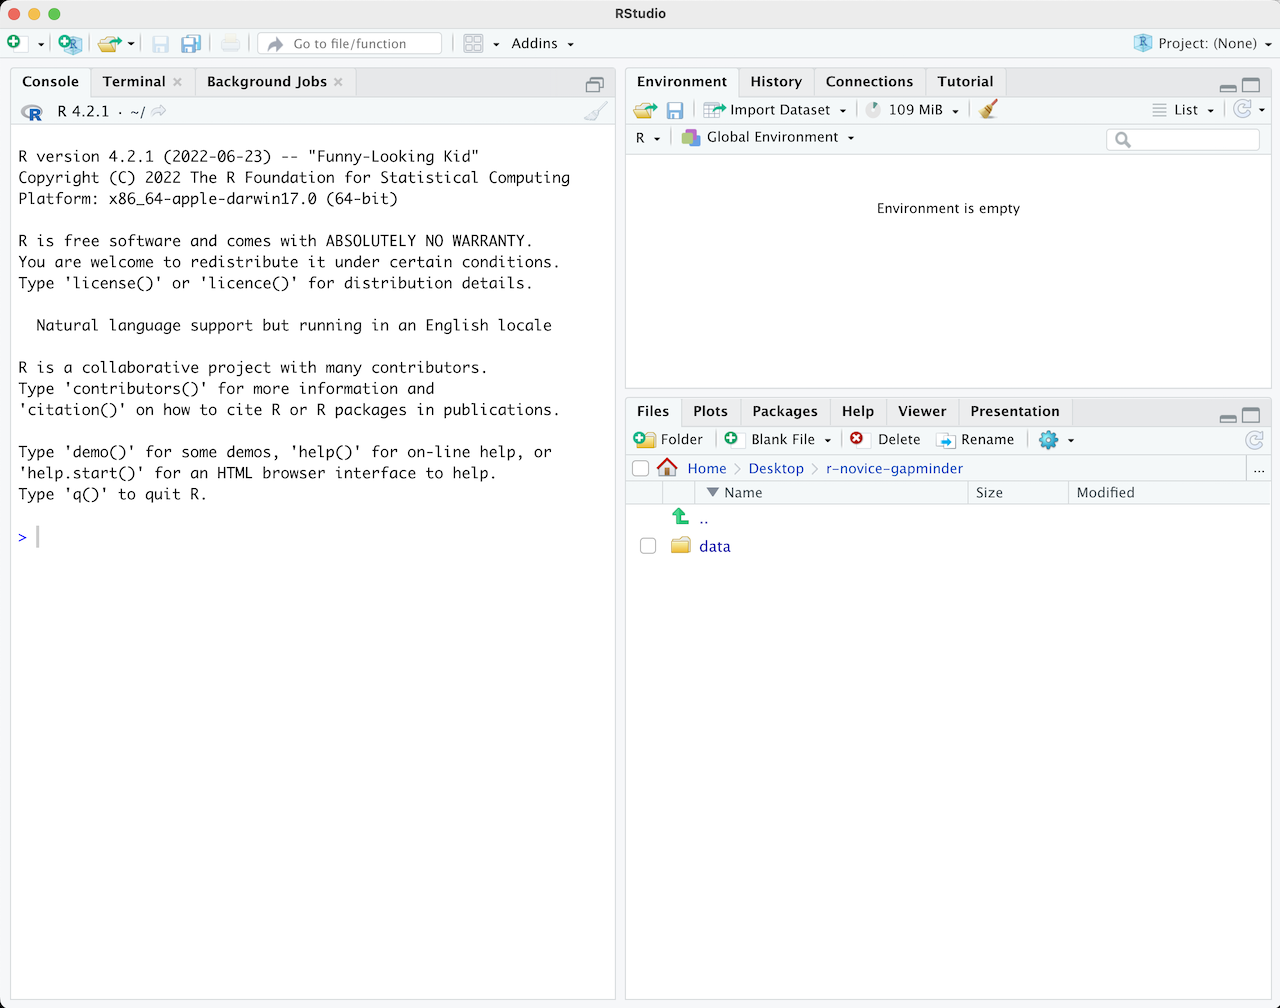
\includegraphics[width=0.7\textwidth]{images/01-rstudio.png}
  \label{fig:rstudio}
 \caption{L'interfaccia di RStudio con i tre pannelli che si vedono alla prima apertura del programma. La colonna di sinistra \`e interamente occupata dalla console (o terminale) interattivo, mentre la colonna di destra \`e divisa in due pannelli, in alto quello che elenca il contenuto dell'ambiente di lavoro e la storia dei comandi eseguiti, in basso quello che mostra il filesystem, i grafici che andremo a creare, e i messaggi di aiuto.}
\end{figure}


\begin{figure}[h!]
 \centering
  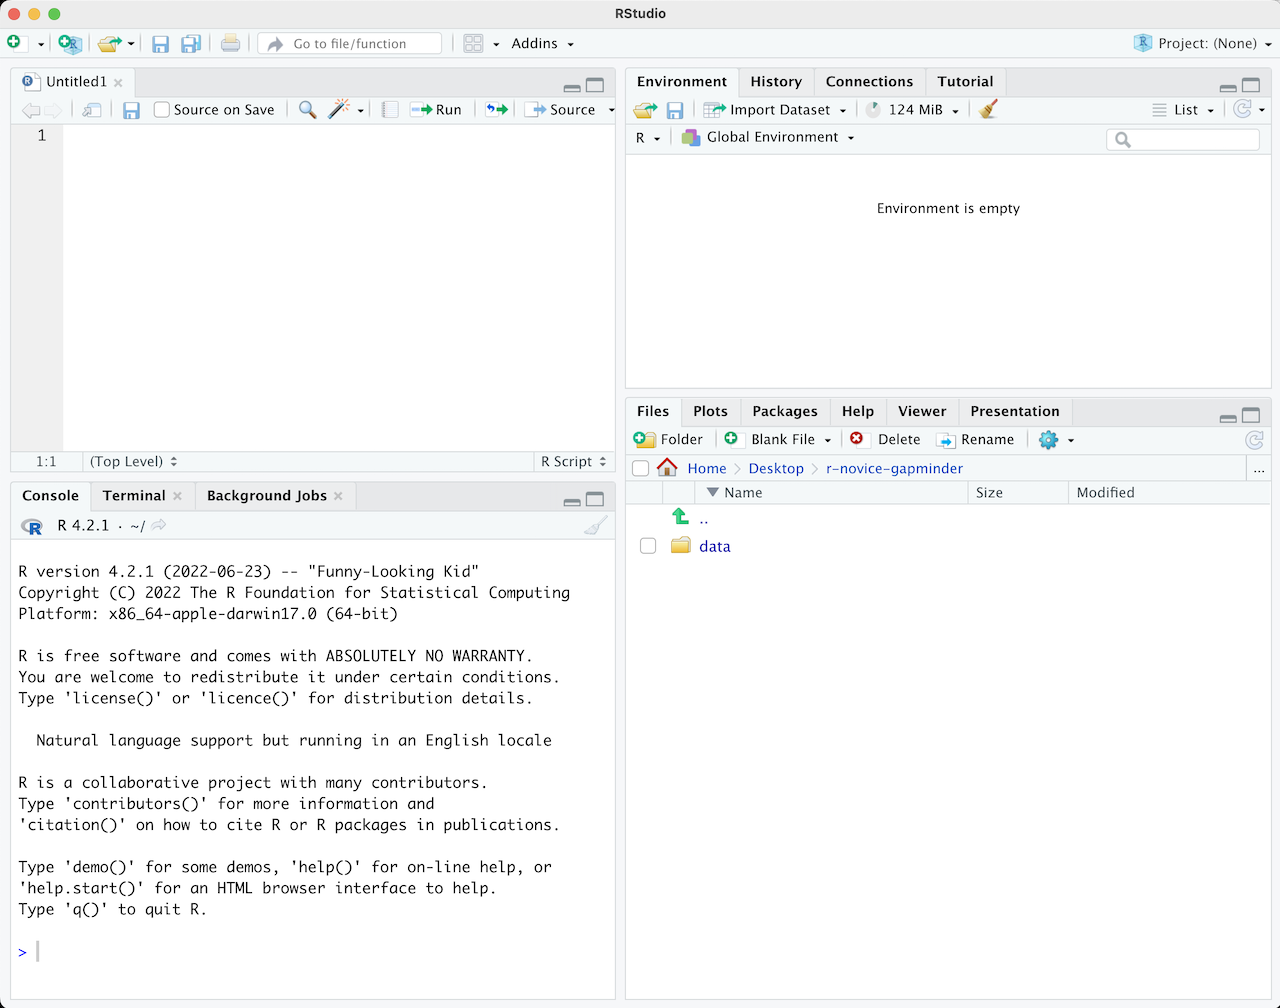
\includegraphics[width=0.7\textwidth]{images/01-rstudio-script.png}
   \label{fig:rstudio-script}
 \caption{L'interfaccia di RStudio con tutti e quattro i pannelli. Rispetto a Figure~\ref{fig:rstudio}, vediamo in alto a sinistra il pannello per la modifica degli script R. Il pannello con la console interattiva viene ridotto in basso a sinistra.}
\end{figure}


\section{Usare R come una calcolatrice}

La cosa pi\`u semplice che si pu\`o fare con R sono i calcoli aritmetici. Per esempio, se scrivete nella console:

\begin{lstlisting}[style=Rstyle]
1 + 100
\end{lstlisting}
%
e premete \lsin{Invio} (sulla tastiera) otterrete il seguente risultato

\begin{lstlisting}[style=Rstyle]
[1] 101
\end{lstlisting}
%
dove \lsin{[1]} rappresenta l'indice del primo elemento stampato in una linea della console (vedremo qualche esempio chiarificatore pi\`u aventi). 

\noindent
Se premete invio prima di completare un comando, R aspetter\`a che voi lo completiate. Per esempio, se scrivete

\begin{lstlisting}[style=Rstyle]
1 + 
\end{lstlisting}
%
e premete \lsin{Invio}, otterrete il seguente output

\begin{lstlisting}[style=Rstyle]
+ 
\end{lstlisting}
%
In generale, ogni volta che la sessione (riga nella console) mostra un \lsin{+} invece che un \lsin{>} vuol dire che R sta attendendo che voi completiate il comando -- se volete ritornare alla console, premete \lsin{ESC} sulla tastiera. Un'altra strategia \`e premere \lsin{Ctrl+C}. Questa seconda opzione vi permette anche di interrompere l'esecuzione di uno o pi\`u comandi, per esempio perch\'e sono molto (troppo) lunghi da eseguire o perch\'e  avete notato un errore nel codice. 


\subsection{L'ordine delle operazioni}

L'ordine in cui le operazioni aritmetiche sono svolte \`e quello classico, cio\`e (in ordine di precedenza):

\begin{myenumerate}
	\item parentesi: \lsin{()}
	\item esponenti: \lsin{^} oppure \lsin{**}
	\item moltiplicazioni: \lsin{*}
	\item divisioni: \lsin{/}
	\item addizioni: \lsin{+}
	\item sottrazioni: \lsin{-}
\end{myenumerate}	

\noindent Se scriviamo sulla console:

\begin{lstlisting}[style=Rstyle]
3 + 5 * 2
\end{lstlisting}
%
otteniamo:

\begin{lstlisting}[style=Rstyle]
[1] 13
\end{lstlisting}
%
Perci\`o, se l'ordine di esecuzione \`e diverso da quello di default, o anche sono per chiarezza, \`e meglio utilizzare le parentesi:

\begin{lstlisting}[style=Rstyle]
(3 + 5) * 2
\end{lstlisting}
%
otteniamo:
\begin{lstlisting}[style=Rstyle]
[1] 16
\end{lstlisting}
%
Attenzione al modo in cui scrivete le operazioni e usate le parentesi: il codice potrebbe diventare illeggibile sia per voi che per altri. Per esempio:

\begin{lstlisting}[style=Rstyle]
(3 + (5 * (2 ^ 2))) # difficile da leggere
3 + 5 * 2 ^ 2       # chiaro, se ci si ricorda le regole
3 + 5 * (2 ^ 2)     # chiaro anche se non ricordiamo le regole
\end{lstlisting}
%
sono equivalenti:
\begin{lstlisting}[style=Rstyle]
[1] 23
\end{lstlisting}

\subsection{I commenti nel codice}

L'hash (\lsin{#} indica l'inizio di un commento, ovvero una stringa che viene ignorata da R e serve al programmatore/analista per capire cosa il codice stia facendo. Qualsiasi cosa che venga scritta dopo un \lsin{#} viene ignorata da R.

\subsection{La notazione scientifica}

Numeri molto grandi (o molto piccoli) vengono trasformati in notazione scientifica:

\begin{lstlisting}[style=Rstyle]
2/100000
[1] 2e-05
\end{lstlisting}

\begin{lstlisting}[style=Rstyle]
2*100000
[1] 2e+05
\end{lstlisting}
%
dove \lsin{e-05} vuol dire moltiplica per $10^{-5}$. Quindi, \lsin{2e-05} vuol dire $2 \times 10^{-5}$ e  \lsin{2e+05} vuol dire $2 \times 10^{5}$.



\section{Funzioni matematiche (e non solo)}
\label{sec:Rfunctions}

R offre una serie di funzioni matematiche ma anche (e non solo) di sistema. Le funzioni si invocano digitando il loro nome, seguite da aperta chiusa parentesi tonda. Alcune funzioni prendono uno o pi\`u argomenti, che andremo a inserire all'interno delle parentesi, separati da virgole.


\noindent Per esempio:

\begin{lstlisting}[style=Rstyle]
sqrt(9) # radice quadrata
[1] 3
\end{lstlisting}
%
prende un argomento, il numero di cui vogliamo fare la radice quadrata.

\begin{lstlisting}[style=Rstyle]
round(33.333333, 1) # arrotondamento
[1] 33.3
\end{lstlisting}
%
prende due argomenti, il primo argomento \`e il numero che deve essere arrotondato in modo che abbia tante cifre decimali quanto specificato dal secondo argomento.

\begin{lstlisting}[style=Rstyle]
ls() # lista
\end{lstlisting}
%
non prende nessun argomento e ci stampa tutti gli oggetti che sono presenti nel nostro ambiente (lo vedremo pi\`u nel dettaglio in Sezione~\ref{sec:environment}).

\noindent Non vi preoccupate se non ricordate il nome di una funzione: Google \`e vostro amico, e se ne ricordate almeno l'inizio potete usare l'auto-completamento con il \lsin{TAB} (sulla tastiera).


\section{Chiedere aiuto}

In generale, se si digita \lsin{?} prima del nome di una funzione (per esempio: \lsin{?function_name}) si aprir\`a la sua pagina di aiuto nel pannello in basso a destra di RStudio. Un comando analogo \`e \lsin{help(function_name)}.

\begin{lstlisting}[style=Rstyle]
?round
\end{lstlisting}

\noindent La pagina di aiuto contiene una descrizione dettagliata del comando e dei suoi argomenti, seguito, spesso, da un esempio di codice che illustra come deve essere usato. In generale, queste sono le sezioni pi\`u utili che trovate nella pagina di aiuto: 

\begin{myitemize}
\item    \emph{Description:} una descrizione pi\`u o meno estesa di cosa faccia una funzione 
\item    \emph{Usage:} gli argomenti di una funzione, con eventuali parametri di default (che possono essere modificati) 
\item    \emph{Arguments: } informazioni pi\`u dettagliate sul tipo di dati che ciascun argomento si aspetta
\item    \emph{Details: } qualsiasi dettaglio che lo sviluppatore ha ritenuto utile evidenziare
\item    \emph{Value:} il tipo di dati restituito in output dalla funzione
\item    \emph{Examples:} esempi di uso della funzione. In RStudio, se li evidenziate e premete \lsin{Ctrl+Return} potete eseguirli nella console.
\end{myitemize}


\noindent Se non vi ricordate il nome esatto di una funzione potete usare l'operatore \lsin{??} per fare una ricerca approssimata. Per esempio, se vi ricordate che include la parola \lsin{set} potete usare:

\begin{lstlisting}[style=Rstyle]
??set
\end{lstlisting}
%
per visualizzare, nel pannello in basso a destra di RStudio, un elenco di funzioni che la contengano.


\section{Comparare oggetti}

\begin{lstlisting}[style=Rstyle]
1 == 1  # uguale a?
[1] TRUE
1 == 2  # uguale a?
[1] FALSE

1 != 1  # diverso da?
[1] FALSE
1 != 2  # diverso da?
[1] TRUE

1 < 2   # Minore di?
[1] TRUE

1 <= 1  # Minore o uguale a?
[1] TRUE

1 >= -2 # Maggiore o uguale a?
[1] TRUE
\end{lstlisting}


\subsection{Comparare variabili continue}

Il \emph{numeri a virgola mobile} sono il modo in cui un calcolatore rappresenta delle (approssimazioni) dei numeri reali. Visto che sono delle approssimazioni, alcune cose che ci paiono ovvie, diventano molto meno ovvie:


\begin{lstlisting}[style=Rstyle]
0.1 + 0.05 
[1] 0.15

0.1 + 0.05 == 0.15 
[1] FALSE
\end{lstlisting}
%
Per ovviare a questo problema, quando si vogliono comparare numeri a virgola mobile, si usa la funzione \lsin{all.equal}:

\begin{lstlisting}[style=Rstyle]
all.equal(0.1 + 0.05, 0.15)
[1] TRUE
\end{lstlisting}


\section{Variabili}

Per assegnare un valore a una variabile si possono usare due notazioni, la freccia (\lsin{<-}), che \`e lo standard in R, o il singolo simbolo di uguale (\lsin{=})\footnote{Attenzione a non confonderlo con il doppio simbolo di uguale \lsin{==} che viene usato per comparare due oggetti.}:

\begin{lstlisting}[style=Rstyle]
x <- 1
y = 1
\end{lstlisting}
%
Notiamo che l'operazione di assegnazione non stampa nulla a video. Per visualizzare il valore di una variabile dobbiamo scriverne il nome a terminale:

\begin{lstlisting}[style=Rstyle]
x
[1] 1
y
[1] 1
\end{lstlisting}

\noindent
Se guardate nel pannello in alto a destra di RStudio, vedrete che una variabile \lsin{x} e una \lsin{y} sono apparse insieme al loro valore.

\vspace{0.2cm}

\noindent
Le variabili possono essere usate in vece dei valori che rappresentano:

\begin{lstlisting}[style=Rstyle]
z <- 9

sqrt(z)
[1] 3

sqrt(z) + 1
[1] 4
\end{lstlisting}
%
Le variabili possono anche essere riassegnate, sia con nuovi valori sia con i valori contenuti da altre variabili sia con i risultati di operazioni tra variabili:

\begin{lstlisting}[style=Rstyle]
x <- 4
y <- x
z <- sqrt(y) + x

x
[1] 4
y
[1] 4
z
[1] 6
\end{lstlisting}

\noindent In R\footnote{Altri linguaggi di programmazione possono seguire regole diverse.}, il nome di una variabile non pu\`o mai iniziare con un numero o con un underscore (\lsin{_}) n\'e contenere spazi o trattini (\lsin{-}). Variabili che iniziano con un punto, sono variabili ``nascoste''. 

\begin{mybox}{Variabile (informatica)}
In informatica, il termine variabile indica un ``contenitore'' un cui sono contenuti dei valori che possono o meno essere modificati durante l'esecuzione di un programma.

La variabile \`e definita da un ``nome'', ovvero una sequenza di lettere o numeri. \`E consigliabile che il nome della variabile rappresenti il suo contenuto, per esempio, \lsin{weight, height, BMI}. In caso di nomi lunghi, ci sono diverse strategie: 
\lsin{periods.between.words} (considerato il classico in R),
\lsin{underscores_between_words} (pi\`u leggibile), e
\lsin{camelCaseToSeparateWords} (meno leggibile).

Attenzione a non confondere variabili (il contenitore) con i valori (il contenuto).
\end{mybox}


\vspace{0.5cm} 

\begin{exercise}\label{ex2.1}

\noindent
Quali dei seguenti nomi di variabile sono validi in R?

\begin{lstlisting}[style=Rstyle]
min_height
max.height
_age
.mass
MaxLength
min-length
2widths
celsius2kelvin
\end{lstlisting}

	\exnote{Suggerimenti}%
	\begin{myitemize}
		\item provate a assegnare loro un valore 
	\end{myitemize}
\end{exercise}


\vspace{0.5cm} 

\begin{exercise}\label{ex2.2}

\noindent
Quale sar\`a il valore delle variabili \lsin{x} e \lsin{y} dopo che il seguente codice \`e stato eseguito?

\begin{lstlisting}[style=Rstyle]
x <- 50.5
y <- 122
x <- x * 2
y <- y - 20
\end{lstlisting}
	
\end{exercise}	


\vspace{0.5cm} 

\begin{exercise}\label{ex2.3}

\noindent
Scrivi un comando per capire se \lsin{x} sia pi\`u grande di \lsin{y}.

\end{exercise}	


\section{Gestire l'ambiente R}
\label{sec:environment}

Ci sono alcuni comandi molto utili per interagire con l'ambiente R.

\begin{lstlisting}[style=Rstyle]
ls()
[1] "x" "y" "z"
\end{lstlisting}
%
elenca (in ordine alfanumerico) tutte le variabili e funzioni che sono caricate nella vostra sessione di lavoro (o \emph{global environment})
%
Attenzione alle variabili nascoste, ovvero quelle che iniziano per \lsin{.}: per elencarle dovrete usare la funzione \lsin{ls} con il parametro \lsin{all.names=TRUE}

\begin{lstlisting}[style=Rstyle]
.hidden <- "nascosta"

ls()
[1] "x" "y" "z"

ls(all.names=TRUE)
[1] ".hidden" "x" "y" "z"
\end{lstlisting}
%
Quando assegniamo il valore a un parametro (l'argomento di una funzione, vedi sezione~\ref{sec:Rfunctions}) dobbiamo usare l'operatore \lsin{=}. Se si usa \lsin{<-} ci potrebbero essere dei side effects, o, pi\`u probabilmente un messaggio di errore:

\begin{lstlisting}[style=Rstyle]
ls(all.names <- TRUE)
(*@\textbf{\textcolor{red}{ Error in as.environment(pos) : invalid object for 'as.environment' }}@*)
\end{lstlisting}

\begin{mybox}{Warnings vs Errors}
	
Un errore indica che R non pu\`o proseguire con la computazione. Warnings, invece, indicano che la funzione \`e stata eseguita, ma probabilmente non ha funzionato come previsto. In entrambi i casi, R stampa a video un messaggio che dovrebbe aiutarvi a capire cosa \`e successo (o da copiare e incollare su Google, per quello che \`e importante installare R in inglese). In entrambi i casi, R vi segnala che c'\`e un problema che non dovreste ignorare.

\end{mybox}


\noindent Un altro comando utile per gestire con l'ambiente R \`e \lsin{rm()}, che elimina una o pi\`u variabili dall'ambiente di lavoro:

\begin{lstlisting}[style=Rstyle]
ls()
[1] "x" "y" "z"

rm(x)

ls()
[1] "y" "z"
\end{lstlisting}
%
Se avete molte variabili e le volete eliminare tutte, potete passare il loro elenco, come generato da \lsin{ls()} come parametro di \lsin{rm()}:

\begin{lstlisting}[style=Rstyle]
ls()
[1] "y" "z"

rm(list = ls())

ls()
character(0)
\end{lstlisting}
%
Attenzione: non potete pi\`u ripristinare una variabile eliminata. Come con i diamanti, un \lsin{rm} \`e per sempre.


\noindent Se quando chiamate una funzione vi dimenticate di aggiungere le parentesi dopo il nome, R stampa a video il codice della funzione stessa

\begin{lstlisting}[style=Rstyle]
rm

function (..., list = character(), pos = -1, envir = as.environment(pos), 
    inherits = FALSE) 
{
    if (...length()) {
        dots <- match.call(expand.dots = FALSE)$...
        if (!all(vapply(dots, function(x) is.symbol(x) || is.character(x), 
            NA, USE.NAMES = FALSE))) 
            stop("... must contain names or character strings")
        list <- .Primitive("c")(list, vapply(dots, as.character, 
            ""))
    }
    .Internal(remove(list, envir, inherits))
}
<bytecode: 0x1265d4d60>
<environment: namespace:base>
\end{lstlisting}
%
Perch\'e lo fa? Per R, chiamare qualcosa per nome indica la volont\`a dell'utente di stamparne il contenuto a video, sia questa una variabile numerica, una stringa di caratteri o una funzione.


\vspace{0.5cm} 

\begin{exercise}\label{ex2.4}

\noindent
Scrivi i comandi per creare due variabili \lsin{mass} e \lsin{age}, assegnare loro i valori 2.2 e 15, e poi rimuoverli dall'ambiente di lavoro.

\end{exercise}	

\noindent Sapere in che cartella ci troviamo \`e importante perch\`e quando dobbiamo accedere ad altri file (per esempio caricare dei dati, come vedremo in Sezione~\ref{sec:data_loading}) R andr\`a a cercarli in relazione alla cartella corrente.

\begin{lstlisting}[style=Rstyle]
# Visualizza la cartella corrente
getwd()
[1] "/Users/visconti/"

# Seleziona la cartella di lavoro
setwd("~/Desktop")

# Visualizza la cartella corrente
getwd()
[1] "/Users/visconti/Desktop/"
\end{lstlisting}

\begin{mybox}{Il filesystem}	

Il filesystem \`e la parte di un Sistema Operativo che \`e responsabile della gestione di file e cartelle. I file sono oggetti che contengono informazioni (testo, immagini, video, musica, programmi, \dots), e le cartelle sono oggetti che contengono file e/o altre cartelle. 

\noindent Le cartelle permettono di organizzare il contenuto del nostro computer in modo gerarchico, attraverso una struttura ad albero. Si parte dalla cartella principale detta ROOT (radice, indicata per esempio con \lsin{C:\} o \lsin{/} in Linux/Mac OS X), che contiene file e cartelle di secondo livello, che a loro volta conterranno altri file e cartelle di terzo livello e cos\`i via, in una serie di livelli annidati uno dentro l’altro.

\noindent La posizione di un file o di una cartella nel filesystem, e di conseguenza il percorso che bisogna fare per raggiungerli, pu\`o essere assoluto o relativo. Il percorso assoluto parte dalla cartella root. Il percorso relativo parte dalla cartella in cui ci troviamo (relativamente a essa per l'appunto) e sale o scende lungo l'albero delle cartelle.

\end{mybox}


\section{Pacchetti R}
\label{sec:R_package}

R \`e molto versatile perch\'e esistono moltissimi pacchetti (insiemi di funzioni, anche chiamate \emph{librerie}) che ci permettono di fare le cose pi\`u disparate.

\noindent I comandi R per gestire i pacchetti sono:

\begin{myitemize}
	\item \lsin{installed.packages()} visualizza i pacchetti installati
	\item \lsin{install.packages("packagename")} installa un pacchetto (attenzione alle virgolette doppie)
	\item \lsin{update.packages()} aggiorna i pacchetti installati
	\item \lsin{remove.packages("packagename")} disinstalla un pacchetto (attenzione alle virgolette doppie)
\end{myitemize}

\noindent Per poter usare un pacchetto (che sia stato precedentemente installato) serve caricarlo ad ogni sessione o all'inizio dello script che lo usa usando il comando \lsin{library(packagename)}.



\vspace{0.5cm} 

\begin{exercise}\label{ex2.5}

\noindent Installare il pacchetto R \lsin{ggplot2} utilizzando il seguente comando: 

\begin{lstlisting}[style=Rstyle]
install.packages("ggplot2", dependencies = TRUE)
\end{lstlisting}
%
Che comando usiamo per caricarlo nella sessione di lavoro?

\noindent Installate ora il pacchetto \lsin{ggrepel}.

\end{exercise}	


\vspace{0.5cm}

\begin{tcolorbox}[width=1\linewidth, halign=left, colframe=blue!60, colback=white, boxsep=1mm, arc=3mm]

\textbf{Punti principali}

\begin{myitemize}
    \item Usare  R per semplici operazioni aritmetiche e logiche
    \item Usare \lsin{<-} per assegnare un valore a una variabile
    \item Usare \lsin{ls()} per elencare le variabili in un ambiente di lavoro 
    \item Usare \lsin{rm()} per rimuovere una o pi\`u variabili dall'ambiente di lavoro 
    \item Usare \lsin{install.packages()} per installare un pacchetto R
	\item Usare \lsin{?, ?? o help()} per chiedere aiuto 
\end{myitemize}

\end{tcolorbox} 


\chapter{Dati \& strutture dati}
\label{cap:dati}

\section*{Obiettivi di apprendimento}


\begin{multicols}{2}
\begin{tcolorbox}[width=1\linewidth, halign=left, colframe=blue!60, colback=white, boxsep=1mm, arc=3mm]

Domande

\begin{myitemize}
	\item Come posso leggere i dati in R?
	\item Quali sono i tipi di dati disponibili in R?
	\item Cos'\`e un data frame e come lo posso manipolare?
\end{myitemize}

\end{tcolorbox} 
\columnbreak
\begin{tcolorbox}[width=1\linewidth, halign=left, colframe=blue!60, colback=white, boxsep=1mm, arc=3mm]

Obiettivi

\begin{myitemize}
	\item Riconoscere i tipi di dato disponibili in R
	\item Riconoscere i tipi di strutture dato disponibili in R
	\item Saper creare e modificare un data frame
	\item Saper estrarre parti di un vettore e/o di un data frame usando indici, nomi o operatori di comparazione
\end{myitemize}

\end{tcolorbox} 
\columnbreak
\end{multicols}


\section{Caricare i dati in R}
\label{sec:data_loading}

Uno dei pi\`u importanti vantaggi di R \`e la sua abilit\`a nel gestire dati tabulari (come quelli contenuti in un foglio di lavoro Excel). 

\noindent Iniziamo quindi a lavorare con dei dati tabulari che rappresentano una versione pi\`u piccola del dataset che useremo nel resto delle dispense, che sono a disposizione online. 

\noindent Il primo passo \`e andarli a scaricare in una cartella locale utilizzando la funzione \lsin{download.file()}:

\begin{lstlisting}[style=Rstyle]
# L'indirizzo dal quale scaricare i dati
url <- "https://t.ly/02JL_"

# Il nome del file e dove salvarlo nel proprio computer
filename <- "gapminder_small.csv"
filepath <- "~/Desktop/Rlab/data/"

# Se la cartella non esiste la dobbiamo creare
dir.create(filepath, recursive = TRUE)

# Scarica il file
download.file(url, paste(filepath, filename, sep=""), mode = "w")
(*@\textbf{\textcolor{red}{trying URL 'https://t.ly/is5J6' }}@*)
(*@\textbf{\textcolor{red}{Content type 'text/plain; charset=utf-8' length 450 bytes }}@*)
(*@\textbf{\textcolor{red}{================================================== }}@*)
(*@\textbf{\textcolor{red}{downloaded 450 bytes }}@*)


# Entriamo nella nostra cartella e verifichiamo che il file esista
setwd(filepath)

# Controlliamo di essere dove pensiamo di essere
getwd()
[1] "/Users/visconti/Desktop/Rlab/data"

# Visualizza il contenuto di una cartella
dir()
[1] "gapminder_small.csv"
\end{lstlisting}



\noindent Dopo che il file \`e disponibile, possiamo finalmente caricarlo nell'ambiente R e visualizzarlo:

\begin{lstlisting}[style=Rstyle]
df <- read.csv("gapminder_small.csv")

df
      country world_region income_group_2017
1       Benin       africa        Low income
2      Greece       europe       High income
3    Tanzania       africa        Low income
4     Estonia       europe       High income
5      Russia       europe     Middle income
6       Syria         asia     Middle income
7      Zambia       africa     Middle income
8     Vietnam         asia     Middle income
9     Liberia       africa        Low income
10 Mozambique       africa        Low income
   happiness_score_2011 gov_health_spending_percent
1                  38.7                        9.60
2                  53.7                       12.10
3                  40.7                       13.80
4                  54.9                       11.70
5                  53.9                        8.04
6                  40.4                        5.58
7                  50.0                       15.60
8                  57.7                        7.79
9                    NA                       11.10
10                 49.7                       12.20
\end{lstlisting}
%
Notiamo la presenza di un valore indicato con \lsin{NA} (Not Available): indica un dato mancante, che non era disponibile nei nostri dati. A volta la presenza di \lsin{NA} crea dei problemi, vedremo come risolverne alcuni. Non confondetelo con \lsin{NULL}, che rappresenta un valore che non esiste, non un valore che esiste e non \`e conosciuto\footnote{R ha altri tipi di variabile che indicano dei "concetti" piuttosto che dei valori. Per esempio, \lsin{NaN} (Not a Number) indica un valore non possibile, come quello che si otterrebbe dividendo per zero, \lsin{Inf/-Inf} che indicano numeri troppo grandi/piccoli per essere rappresentati in R.}.

\vspace{0.2cm}

\noindent  Una volta che il file \`e stato caricato possiamo iniziare ad usarlo, per esempio estraendone una colonna utilizzando l'operatore \lsin{$}. 

\begin{lstlisting}[style=Rstyle]
df$country
 [1] "Benin"      "Greece"     "Tanzania"   "Estonia"    "Russia"    
 [6] "Syria"      "Zambia"     "Vietnam"    "Liberia"    "Mozambique"
	
df$happiness_score_2011
[1] 38.7 53.7 40.7 54.9 53.9 40.4 50.0 57.7   NA 49.7
\end{lstlisting}
%
Se chiedessimo il valore di un attributo che non esiste, per esempio \lsin{total_spending} otterremmo un \lsin{NULL}, che appunto indica qualcosa che non esiste:

\begin{lstlisting}[style=Rstyle]
df$total_spending
NULL
\end{lstlisting}

\noindent Le colonne che abbiamo estratto possono anche essere usate per delle operazioni:

\begin{lstlisting}[style=Rstyle]	
# Concatenare stringhe	
paste(df$country, "is in", df$world_region)
[1] "Benin is in africa"      "Greece is in europe"    
[3] "Tanzania is in africa"   "Estonia is in europe"   
[5] "Russia is in europe"     "Syria is in asia"       
[7] "Zambia is in africa"     "Vietnam is in asia"     
[9] "Liberia is in africa"    "Mozambique is in africa"

# Fare operazioni aritmentiche
df$happiness_score_2011/100
 [1] 0.387 0.537 0.407 0.549 0.539 0.404 0.500 0.577
 [9]    NA 0.497

# Concatenare stringhe e numeri
paste("The happiness score of", df$country, "is", df$happiness_score_2011)
 [1] "The happiness score of Benin is 38.7"     
 [2] "The happiness score of Greece is 53.7"    
 [3] "The happiness score of Tanzania is 40.7"  
 [4] "The happiness score of Estonia is 54.9"   
 [5] "The happiness score of Russia is 53.9"    
 [6] "The happiness score of Syria is 40.4"     
 [7] "The happiness score of Zambia is 50"      
 [8] "The happiness score of Vietnam is 57.7"   
 [9] "The happiness score of Liberia is NA"     
[10] "The happiness score of Mozambique is 49.7"
\end{lstlisting}


\section{I tipi di dato in R}

Abbiamo appena visto come fare delle operazioni, ma cosa succede se facciamo:

\begin{lstlisting}[style=Rstyle]	
# Dividiamo happiness score per il paese	
df$happiness_score_2011/df$country
(*@\textbf{\textcolor{red}{Error in df$happiness_score_2011/df$country :  }}@*)
(*@\textbf{\textcolor{red}{  non-numeric argument to binary operator }}@*)
\end{lstlisting}
%
R ci sta dicendo, in modo un po' oscuro, che dividere un valore numerico (l'happiness score) per una stringa (il paese) non ha senso. 

\noindent In R per scoprire il tipo di una variabile si pu\`o usare \lsin{class()} o \lsin{typeof()}. La differenza tra i due \`e che il primo \`e pi\`u flessibile \`e pu\`o essere esteso includendo anche le strutture dati (che vedremo tra breve), mentre il secondo ritorna solo uno dei principali tipo di dato usati da R: \lsin{numeric} (o \lsin{double}), \lsin{integer, complex, logical} e \lsin{character}. 

\begin{lstlisting}[style=Rstyle]	
class(df$happiness_score_2011)
[1] "numeric"

typeof(df$happiness_score_2011)
[1] "double"

class(df$country)
[1] "character"

typeof(df$country)
[1] "character"

class(TRUE)
[1] "logical"

typeof(TRUE)
[1] "logical"

class(df)
[1] "data.frame"
\end{lstlisting}
%
Un \lsin{data.frame} non \`e un tipo di dato, ma un tipo di struttura dati\footnote{Se faceste \lsin{typeof(df)}, otterreste \lsin{list}, che \`e un altro tipo di struttura dati.}.

\section{I data frame}

I data frame sono una delle strutture dati pi\`u versatili\footnote{Insieme alle liste, che non vedremo nel dettaglio in questo corso.}e sono formati da righe e colonne.

\noindent Andiamo a crearne uno molto semplice:

\begin{lstlisting}[style=Rstyle]
cats <- data.frame(coat = c("calico", "black", "tabby"),
                   weight = c(2.1, 5.0, 3.2),
                   playful = c(1, 0, 1))
				   
cats					
    coat weight  playful
1 calico    2.1        1
2  black    5.0        0
3  tabby    3.2        1
\end{lstlisting}

\vspace{0.2cm}

\noindent Differenti colonne di un data frame possono essere di tipo diverso, come nell'esempio che abbiamo esplorato sino ad ora, ma una colonna pu\`o essere composta solo da un tipo di dati, che viene deciso al momento del caricamento (o della definizione del data frame), usando il tipo di dati meno restrittivo. Per esempio se avessimo un data.frame cos\`i composto:

\begin{lstlisting}[style=Rstyle]	
cats2 <- data.frame(coat = c("calico", "black", "tabby"),
                    weight = c(2.1, 5.0, "3.2kg"),
                    playful = c(1, 0, 1))	
	
cats2
    coat   weight  playful
1 calico      2.1        1
2  black      5.0        0
3  tabby    3.2kg        1

class(cats2$weight)
[1] "character"
\end{lstlisting}
%
perch\'e \lsin{2.1, 5.0} possono essere interpretati come \lsin{"character"}, ma \lsin{3.2kg} non pu\'o essere interpretato come \lsin{numeric}.

\noindent La struttura di un data frame pu\`o essere visualizzata con la funzione \lsin{str()}:

\begin{lstlisting}[style=Rstyle]	
str(cats)
'data.frame'  :	3 obs. of  3 variables:
 $ coat       : chr  "calico" "black" "tabby"
 $ weight     : num  2.1 5 3.2
 $ playful    : num  1 0 1
\end{lstlisting}

\vspace{0.5cm} 

\begin{exercise}\label{ex3.1}

\noindent \`E possibile accedere a un data frame in diversi modi. Prova i seguenti e spiega cosa ottieni:

\begin{lstlisting}[style=Rstyle]	
    df$country
    df["country"]
    df[1, 1]
    df[, 1]
    df[1, ]
\end{lstlisting}

\end{exercise}


\subsection{Aggiungere righe e colonne}

Una cosa che non abbiamo ancora detto \`e che righe e colonne di un data frame sono vettori (un altro tipo di strutture dati) e che i vettori vengono costruiti concatenando, con la funzione \lsin{c()}, dei valori. Per esempio, se vogliamo aggiungere informazioni sull'et\`a dei nostri gatti:

\begin{lstlisting}[style=Rstyle]	
# Creo un vettore di eta' concatenandone i valori
age <- c(2, 3, 5)
[1] 2 3 5
class(age)
[1] "numeric"

# Concateno il vettore al mio data frame come colonna
cbind(cats, age)
    coat weight  playful age
1 calico    2.1        1   2
2  black    5.0        0   3
3  tabby    3.2        1   5
\end{lstlisting}
%
Attenzione: il numero di righe del data frame e il numero di elementi del vettore devono essere uguali:

\begin{lstlisting}[style=Rstyle]	
wrong.age <- c(2, 3)
cbind(cats, wrong.age)
(*@\textbf{\textcolor{red}{Error in data.frame(..., check.names = FALSE) :  }}@*)
(*@\textbf{\textcolor{red}{  arguments imply differing number of rows: 3, 2  }}@*)
  
wrong.age <- c(2, 3, 5, 7)
cbind(cats, wrong.age)
(*@\textbf{\textcolor{red}{Error in data.frame(..., check.names = FALSE) :   }}@*)
(*@\textbf{\textcolor{red}{  arguments imply differing number of rows: 3, 4  }}@*)
\end{lstlisting}

\noindent Andiamo ora a sovrascrivere il data frame aggiungendo la colonna l'et\`a:

\begin{lstlisting}[style=Rstyle]
age <- c(2, 3, 5)
cats <- cbind(cats, age)

cats
    coat weight  playful age
1 calico    2.1        1   2
2  black    5.0        0   3
3  tabby    3.2        1   5
\end{lstlisting}
%
Andiamo ora a creare una nuova riga:

\begin{lstlisting}[style=Rstyle]
new.cat <- c("white", 3.3, 1, 9)

# Concateno il vettore al mio data frame come riga
cats2 <- rbind(cats, new.cat)

cats2
     coat weight  playful age
1  calico    2.1        1   2
2   black      5        0   3
3   tabby    3.2        1   5
4   white    3.3     TRUE   9
\end{lstlisting}


\vspace{0.5cm} 

\begin{exercise}\label{ex3.2}

\noindent Cosa succede se visualizzo la struttura (e quindi i tipi di data) del data frame \lsin{cats2} con la funzione \lsin{str()}? Perch\'e?

\begin{lstlisting}[style=Rstyle]	
str(cats2)
\end{lstlisting}

\end{exercise}

\noindent Come posso quindi procedere? Utilizzando un'altra struttura dati: le liste. Le liste permettono di creare elenchi di variabili anche di tipo diverso:

\begin{lstlisting}[style=Rstyle]
new.cat <- list("white", 3.3, TRUE, 9)
cats <- rbind(cats, new.cat)

cats
    coat weight playful age
1 calico    2.1       1   2
2  black    5.0       0   3
3  tabby    3.2       1   5
4  white    3.3       1   9

str(cats)
'data.frame': 4 obs. of  4 variables:
 $ coat     : chr  "calico" "black" "tabby" "white"
 $ weight   : num  2.1 5 3.2 3.3
 $ playful  : num  1 0 1 1
 $ age      : num  2 3 5 9
\end{lstlisting}
%
Notiamo che le funzioni \lsin{cbind} e \lsin{rbind} possono essere usate anche per unire due data frame:

\begin{lstlisting}[style=Rstyle]
# Concateno due data frame per colonna		
cbind(cats, cats)
    coat weight playful age   coat weight playful age
1 calico    2.1       1   2 calico    2.1       1   2
2  black    5.0       0   3  black    5.0       0   3
3  tabby    3.2       1   5  tabby    3.2       1   5
4  white    3.3       1   9  white    3.3       1   9
\end{lstlisting}

\begin{lstlisting}[style=Rstyle]
# Concateno due data frame per riga	
    coat weight playful age
1 calico    2.1       1   2
2  black    5.0       0   3
3  tabby    3.2       1   5
4  white    3.3       1   9
5 calico    2.1       1   2
6  black    5.0       0   3
7  tabby    3.2       1   5
8  white    3.3       1   9
\end{lstlisting}


\subsection{Rimuovere righe e colonne}
\label{sec:removefromdf}

Se volessimo rimuovere l'ultima riga:

\begin{lstlisting}[style=Rstyle]
cats[-4, ]

cats
    coat weight playful age
1 calico    2.1       1   2
2  black    5.0       0   3
3  tabby    3.2       1   5
\end{lstlisting}
%
Notiamo che non abbiamo scritto nulla dopo la virgola, indicando che vogliamo rimuoverne tutte le colonne. Se volessimo rimuovere la prima e l'ultima riga devo creare un vettore con tutti gli indici che voglio eliminare usando la funzione \lsin{c()}:

\begin{lstlisting}[style=Rstyle]
cats[-c(1, 4), ]

cats
   coat weight playful age
2 black    5.0       0   3
3 tabby    3.2       1   5
\end{lstlisting}

\noindent Possiamo usare la stessa strategia per rimuovere le colonne, per esempio l'ultima:

\begin{lstlisting}[style=Rstyle]
cats[,-4]

cats
    coat weight playful
1 calico    2.1       1
2  black    5.0       0
3  tabby    3.2       1
4  white    3.3       1
\end{lstlisting}


\vspace{0.5cm} 

\begin{exercise}\label{ex3.3}

\noindent Ricordando che \`e possibile creare un data frame in R con la seguente sintassi:


\begin{lstlisting}[style=Rstyle]
mydf <- data.frame(id = c("a", "b", "c"),
                   x = 1:3,
                   y = c(TRUE, TRUE, FALSE))
\end{lstlisting}

\begin{myenumerate}
	\item Create un data frame chiamato \lsin{classe} che contenga le seguenti informazioni su voi stessi: \lsin{<Nome, Cognome, Giorno di Nascita>}
	\item Aggiungete delle righe che contengano le stesse informazioni per due dei vostri vicini
	\item Aggiungete una colonna con la vostra risposta (\lsin{TRUE/FALSE}) alla domanda \emph{Mi servirebbe una pausa?}
\end{myenumerate}

	\exnote{Suggerimenti}%
	\begin{myitemize}
		\item I comandi che vi servono sono \lsin{rbind()} e \lsin{cbind()}
	\end{myitemize}

\end{exercise}


\subsection{Estrarre sottoinsiemi di righe e colonne}
\label{sec:subsetting}

Conoscere e avere padronanza dei diversi operatori che R mette a disposizione per estrarre sottoinsiemi di un data frame \`e molto importante per effettuare analisi dati. Andiamo quindi ad esplorarli utilizzando il nostro data frame iniziale, \lsin{df} e pi\'u nello specifico con un vettore che andiamo a estrarre dalla prima colonna:

\begin{lstlisting}[style=Rstyle]
# Creo una variabile usando la prima colonna del data frame
happiness <- df$happiness_score_2011

# Assegna un nome alla nuova variabile (un vettore)
names(happiness) <- df$country  

happiness
     Benin     Greece   Tanzania    Estonia 
      38.7       53.7       40.7       54.9 
    Russia      Syria     Zambia    Vietnam 
      53.9       40.4       50.0       57.7 
   Liberia Mozambique 
        NA       49.7 
\end{lstlisting}


\noindent Per estrarre un elemento da un vettore, possiamo fornirne l'indice:
\begin{lstlisting}[style=Rstyle]
happiness[1]
Benin 
 38.7 
 
happiness[8]
Vietnam 
   57.7 
\end{lstlisting}
%
L'operatore \lsin{[i]} indica: estrai l'\emph{i}-esimo elemento. Se volessi estrarre una serie di elementi consecutivo, posso usare l'operatore \lsin{:} per effettuare quello che si chiama \emph{vettorizzazione}:

\begin{lstlisting}[style=Rstyle]
1:4
[1] 1 2 3 4

happiness[1:4]
 Benin   Greece Tanzania  Estonia 
  38.7     53.7     40.7     54.9 
\end{lstlisting}
%
Usando la funzione \lsin{c()} posso anche estrarre una serie di elementi non consecutivi, come abbiamo visto in Sezione~\ref{sec:removefromdf}, quando siamo andati a rimuovere pi\`u righe dal nostro data frame:

\begin{lstlisting}[style=Rstyle]
happiness[c(1,3,6,9)]
 Benin Tanzania    Syria  Liberia 
  38.7     40.7     40.4       NA 
\end{lstlisting}
%
Facciamo per\`o attenzione che l'elemento che ci interessa esista, altrimenti R ritornar\`a un \lsin{NA}, senza metterci al corrente di un risultato anomalo\footnote{Dovrebbe segnalarci il problema almeno con un warning, oppure ritornare, coerentemente, un \lsin{NULL} indicando che il valore richiesto non esiste.}:

\begin{lstlisting}[style=Rstyle]
happiness[c(1,3,6,9,12)]
 Benin Tanzania    Syria  Liberia     <NA> 
  38.7     40.7     40.4       NA       NA 
\end{lstlisting}

\vspace{0.2cm}

\noindent Usando un numero negativo, R restituisce tutti gli elementi, tranne quelli indicati (come abbiamo gi\`a visto in Sezione~\ref{sec:removefromdf}):

\begin{lstlisting}[style=Rstyle]
happiness[-(1:4)]
    Russia      Syria     Zambia    Vietnam 
      53.9       40.4       50.0       57.7 
   Liberia Mozambique 
        NA       49.7 
   
# Attenzione alle parentesi
happiness[-1:4]
(*@\textbf{\textcolor{red}{   Error in happiness[-1:4] : only 0's may be mixed with negative subscripts }}@*)
\end{lstlisting}
%
per capire cosa \`e successo \`e necessario ricordare che \lsin{:} \`e una funzione, mentre \lsin{-} \`e un'operazione e come tale ha la precedenza. Quindi coda fa R?

\begin{lstlisting}[style=Rstyle]
-1:4
[1] -1  0  1  2  3  4
\end{lstlisting}
%
che non pu\`o funzionare perch\'e le posizioni di un vettore (e di tutte le altre strutture dati) vengono numerate a partire da \lsin{1}. 


\vspace{0.5cm} 

\begin{exercise}\label{ex3.4}
	
\noindent Dato il seguente codice:

\begin{lstlisting}[style=Rstyle]
x <- c(5.4, 6.2, 7.1, 4.8, 7.5)
names(x) <- c('a', 'b', 'c', 'd', 'e')

x
  a   b   c   d   e
5.4 6.2 7.1 4.8 7.5 
\end{lstlisting}

Proporre almeno due comandi che producano il seguente output:

\begin{lstlisting}[style=Rstyle]
  b   c   d
6.2 7.1 4.8 
\end{lstlisting}
	
\end{exercise}

\noindent Possiamo anche estrarre gli elementi di un vettore usando il loro nome:

\begin{lstlisting}[style=Rstyle]
happiness["Greece"]
Greece 
  53.7
  
happiness[c("Greece", "Mozambique")]
Greece Mozambique 
  53.7       49.7 
  
# Attenzione ai nomi che non esistono  
Greece Mozambique       <NA>
  53.7       49.7         NA
\end{lstlisting}
%
oppure utilizzando l'operatore \lsin, che ci dice se dei valori sono contenuti all'interno di un insieme:

\begin{lstlisting}[style=Rstyle]
# Questo insieme di paesi e' compreso nel mio vettore?	
c("Greece", "Mozambique", "Italy") %in% names(happiness)
[1]  TRUE  TRUE FALSE

# Estraggo i paesi che ho selezionato
happiness[names(happiness) %in% c("Greece", "Mozambique")]
Greece Mozambique 
  53.7       49.7 
\end{lstlisting}
% 
Usare l'operatore \lsin \`e anche robusto alla richiesta di dati che non esistono:
  
\begin{lstlisting}[style=Rstyle]
happiness[names(happiness) %in% c("Greece", "Mozambique", "Italy")]
Greece Mozambique 
  53.7       49.7  
\end{lstlisting}
%
Rimuovere elementi usando il loro nome, per\`o, \`e pi\`u complicato, perch\'e R non sa come fare il "negativo" di una stringa: 

\begin{lstlisting}[style=Rstyle]
happiness[-"Greece"]
(*@\textbf{\textcolor{red}{   Error in -"Greece" : invalid argument to unary operator }}@*)
\end{lstlisting}
%
Si pu\`o per\`o utilizzare l'operatore diverso (\lsin{!=}):

\begin{lstlisting}[style=Rstyle]
happiness[names(happiness) != "Greece"]
     Benin   Tanzania    Estonia     Russia 
      38.7       40.7       54.9       53.9 
     Syria     Zambia    Vietnam    Liberia 
      40.4       50.0       57.7         NA 
Mozambique 
      49.7 
\end{lstlisting}
%
Rimuovere una serie di elementi \`e ancora pi\`u complicato e ci serve di nuovo l'operatore \lsin, questa volta combiato con l'operatore \lsin{!} (\lsin{not}).

\begin{lstlisting}[style=Rstyle]
happiness[!names(happiness) %in% c("Greece", "Mozambique")]
   Benin Tanzania  Estonia   Russia    Syria   Zambia 
    38.7     40.7     54.9     53.9     40.4     50.0 
 Vietnam  Liberia 
    57.7       NA 
\end{lstlisting}

\vspace{0.2cm}

\noindent Un altro modo per estrarre/rimuovere elementi \`e attraverso dei vettori logici (\lsin{TRUE, FALSE}), che \`e esattamente quello che abbiamo fatto quando abbiamo usato l'operatore \lsin:

\begin{lstlisting}[style=Rstyle]
happiness[c(TRUE, FALSE, FALSE, TRUE, FALSE, TRUE, FALSE, FALSE, TRUE, FALSE)]
 Benin Estonia   Syria Liberia
  38.7    54.9    40.4      NA
\end{lstlisting}
%
che sono utili se vogliamo estrarre elementi che corrispondano a uno specifico criterio, per esempio avere un happiness score maggiore di 50:

\begin{lstlisting}[style=Rstyle]
happiness > 50
     Benin     Greece   Tanzania    Estonia 
     FALSE       TRUE      FALSE       TRUE 
    Russia      Syria     Zambia    Vietnam 
      TRUE      FALSE      FALSE       TRUE 
   Liberia Mozambique 
        NA      FALSE 

happiness[happiness > 50]
 Greece Estonia  Russia Vietnam    <NA>
   53.7    54.9    53.9    57.7      NA

# Attenzione agli NA
happiness[happiness > 50 & !is.na(happiness)]
Greece Estonia  Russia Vietnam
  53.7    54.9    53.9    57.7
\end{lstlisting}
%
\lsin{&} indica l'\lsin{AND} logico. Per l'\lsin{OR} si usa \lsin{|}. La funzione \lsin{is.na()} ci dice se un valore sia \lsin{NA} o meno, il \lsin{!} va a negare il risultato di \lsin{is.na()} :

\begin{lstlisting}[style=Rstyle]
is.na(happiness)
     Benin     Greece   Tanzania    Estonia 
     FALSE      FALSE      FALSE      FALSE 
    Russia      Syria     Zambia    Vietnam 
     FALSE      FALSE      FALSE      FALSE 
   Liberia Mozambique 
      TRUE      FALSE 

!is.na(happiness)
     Benin     Greece   Tanzania    Estonia 
      TRUE       TRUE       TRUE       TRUE 
    Russia      Syria     Zambia    Vietnam 
      TRUE       TRUE       TRUE       TRUE 
   Liberia Mozambique 
     FALSE       TRUE 

happiness > 50
     Benin     Greece   Tanzania    Estonia 
     FALSE       TRUE      FALSE       TRUE 
    Russia      Syria     Zambia    Vietnam 
      TRUE      FALSE      FALSE       TRUE 
   Liberia Mozambique 
        NA      FALSE

happiness > 50 & !is.na(happiness)
     Benin     Greece   Tanzania    Estonia 
     FALSE       TRUE      FALSE       TRUE 
    Russia      Syria     Zambia    Vietnam 
      TRUE      FALSE      FALSE       TRUE 
   Liberia Mozambique 
     FALSE      FALSE 
\end{lstlisting}


\vspace{0.5cm} 

\begin{exercise}\label{ex3.5}
	
\noindent Dato il seguente codice:
	
\begin{lstlisting}[style=Rstyle]
x <- c(5.4, 6.2, 7.1, 4.8, 7.5)
names(x) <- c('a', 'b', 'c', 'd', 'e')

x
  a   b   c   d   e
5.4 6.2 7.1 4.8 7.5 
\end{lstlisting}
%
scrivere un comando che ritorni i valori di \lsin{x} compresi tra 4 e 7.

	\exnote{Suggerimenti}%
	\begin{myitemize}
		\item Dovete usare pi\'u operazioni logiche unite tra loro attraverso gli operatori che abbiamo appena visto.
	\end{myitemize}

\end{exercise}

\noindent Adesso possiamo mettere tutto questo assieme andando a lavorare sui data frame (in modo pi\`u sistematico di quanto fatto nell'Esercizio~\ref{ex3.1}). Un data frame \`e un oggetto a due dimensioni a cui posso essere accedere utilizzando l'operatore \lsin{[]} con due indici: uno per le righe e uno per le colonne:

\begin{lstlisting}[style=Rstyle]
df[1:3, ]
   country world_region income_group_2017
1    Benin       africa        Low income
2   Greece       europe       High income
3 Tanzania       africa        Low income
  happiness_score_2011 gov_health_spending_percent
1                 38.7                         9.6
2                 53.7                        12.1
3                 40.7                        13.8
\end{lstlisting}

\begin{lstlisting}[style=Rstyle]
df[, 1:3]
      country world_region income_group_2017
1       Benin       africa        Low income
2      Greece       europe       High income
3    Tanzania       africa        Low income
4     Estonia       europe       High income
5      Russia       europe     Middle income
6       Syria         asia     Middle income
7      Zambia       africa     Middle income
8     Vietnam         asia     Middle income
9     Liberia       africa        Low income
10 Mozambique       africa        Low income
\end{lstlisting}

\begin{lstlisting}[style=Rstyle]
df[1:3, 1:3]
   country world_region income_group_2017
1    Benin       africa        Low income
2   Greece       europe       High income
3 Tanzania       africa        Low income
\end{lstlisting}
%
e con tutti i meccanismi che abbiamo visto per i vettori:

\begin{lstlisting}[style=Rstyle]
df[df$country == "Greece", ]
  country world_region income_group_2017
2  Greece       europe       High income
  happiness_score_2011 gov_health_spending_percent
2                 53.7                        12.1

df[df$country %in% c("Greece", "Mozambique"), ]
      country world_region income_group_2017
2      Greece       europe       High income
10 Mozambique       africa        Low income
   happiness_score_2011 gov_health_spending_percent
2                  53.7                        12.1
10                 49.7                        12.2

df[df$happiness_score_2011 > 50 & !is.na(df$happiness_score_2011), ]
  country world_region income_group_2017
2  Greece       europe       High income
4 Estonia       europe       High income
5  Russia       europe     Middle income
8 Vietnam         asia     Middle income
  happiness_score_2011 gov_health_spending_percent
2                 53.7                       12.10
4                 54.9                       11.70
5                 53.9                        8.04
8                 57.7                        7.79


df[df$happiness_score_2011 > 50 & !is.na(df$happiness_score_2011), 1:3]
  country world_region income_group_2017
2  Greece       europe       High income
4 Estonia       europe       High income
5  Russia       europe     Middle income
8 Vietnam         asia     Middle income
\end{lstlisting}


\vspace{0.5cm} 

\begin{exercise}\label{ex3.6}

\noindent Scrivi i comandi da utilizzare per:

\begin{myenumerate}
	\item estrarre tutti i valori per paesi europei
	\item estrarre tutti i valori per i paesi non nel gruppo "Middle income"
	\item estrarre tutti i valori nella prima, seconda e ultima colonna
	\item estrarre tutti i valori tranne quelli dell'ultima colonna
	\item estrarre la prima, quarta, e quinta colonna per tutti i paesi africani
\end{myenumerate}

\end{exercise}


\vspace{0.5cm}

\begin{tcolorbox}[width=1\linewidth, halign=left, colframe=blue!60, colback=white, boxsep=1mm, arc=3mm]

\textbf{Punti principali}

\begin{myitemize}
    \item Usare \lsin{read.csv} per leggere dati tabulari 
    \item I tipi di dati in R sono \lsin{numeric} (o \lsin{double}), \lsin{integer, complex, logical} e \lsin{character}
	\item Usare \lsin{str(), class()} e \lsin{typeof()} per capire il tipo di dato di una variabile 
	\item Usare \lsin{c()} per creare o aggiungere elementi a un vettore
	\item Usare \lsin{data.frame()} per creare un data frame
	\item Usare \lsin{list()} per creare una lista
    \item Usare \lsin{cbind()} per aggiungere colonne a un data frame 
    \item Usare \lsin{rbind()} per aggiungere righe a un data frame 
    \item Accedere a un sottoinsieme dei dati in un vettore o data frame utilizzando \lsin{[]}, anche in combinazione con \lsin{start:end} e \lsin{c(...)}
\end{myitemize}

\end{tcolorbox}

\chapter{La statistica descrittiva}
\label{cap:descrittiva}


\section*{Obiettivi di apprendimento}


\begin{multicols}{2}
\begin{tcolorbox}[width=1\linewidth, halign=left, colframe=blue!60, colback=white, boxsep=1mm, arc=3mm]

Domande

\begin{myitemize}
	\item Come posso conoscere le propriet\`a di un data frame?
	\item Come si crea ed esegue uno script in RStudio?
	\item Come si costruiscono tabelle di frequenza e contingenza?
	\item Come si calcolano misure di centralit\`a e dispersione?
	\item Come si calcola la correlazione tra due variabili numeriche?
	\item Come si costruiscono bar, mosaic, box e scatter plots e istogrammi?
\end{myitemize}

\end{tcolorbox} 
\columnbreak
\begin{tcolorbox}[width=1\linewidth, halign=left, colframe=blue!60, colback=white, boxsep=1mm, arc=3mm]

Obiettivi

\begin{myitemize}
	\item Mostrare le propriet\`a di un data frame incluso dimensioni, nome degli attributi, e prime/ultime righe 
	\item Salvare i comandi R in uno script
	\item Saper riassumere numericamente e visivamente dati categorici e numerici
	\item Saper identificare relazioni lineari tra variabili numeriche
\end{myitemize}

\end{tcolorbox} 
\columnbreak
\end{multicols}


\section{Creare uno script in RStudio}
\label{sec:Rscript}

Sino a ora ci siamo limitati a usare la console che RStudio ci mette a disposizione. Come abbiamo per\`o accennato in Sezione~\ref{sec:RStudio}, la console non offre nessuna persistenza, ovvero chiudendo RStudio perdiamo tutto il lavoro fatto. Per il resto del corso, useremo invece uno script R\footnote{In realt\`a andremo a usare anche la console per fare dei piccoli test.}, che garantisce che il nostro lavoro sia sempre disponibile assicurando cos\`i la riproducibilit\`a delle nostre analisi.


\begin{mybox}{Script R}	
	
Uno script R \`e un elenco di comandi R che viene salvato in un file che (indovinate un po' che fantasia) finisce con estensione ``.R''. Salvare i comandi in uno script \`e utile per poterli eseguire di nuovo, per esempio utilizzando la funzione \lsin{source()}

\end{mybox}


\noindent Andiamo quindi a creare un nuovo file attraverso il men\`u \lsin{File} $\rightarrow$ \lsin{New file}  $\rightarrow$ \lsin{R script}. Si apre quindi un nuovo pannello in alto a sinistra, che abbiamo gi\`a visto in Figura~\ref{fig:rstudio-script}. 
%
Usiamo ancora un momento la console per creare una cartella dove il nostro script andr\`a salvato:

\begin{lstlisting}[style=Rstyle]
filepath <- "~/Desktop/Rlab/script/"
dir.create(filepath, recursive = TRUE)
\end{lstlisting}
%
Usiamo quindi di nuovo il men\`u di RStudio per salvare il nostro script: \lsin{File} $\rightarrow$ \lsin{Save As}  $\rightarrow$ andiamo dare un nome al nostro  script (\lsin{gapminder_analysis.R}) e andiamo a scegliere la cartella che abbiamo appena creato.


\subsection{Eseguire pezzi di codice in RStudio}	

Per eseguire la linea di codice corrente (quella su cui avete il cursore) o un blocco di codice (che avrete precedentemente evidenziato) potete:

\begin{myitemize}
	\item cliccare sul bottone \lsin{Run} sul pannello dell'editor dello script (rappresentato con un'icona che mostra un documento e una freccia verde)
	\item usare uno delle diverse opzioni \lsin{Run...} nel men\`u \lsin{Code}
	\item premere \lsin{Ctrl+Return} (Windows/Linux) o \lsin{Cmd+Return} (Mac OS X)
\end{myitemize}

\section{Carichiamo ed esploriamo il dataset Gapminder}


Spostiamoci ora nel pannello dello script\footnote{Per il codice da salvare nello script, lo sfondo passa dal grigio al bianco.}, e andiamo a scrivere il codice per scaricare il dataset che useremo nel resto delle dispense, che avete di nuovo a disposizione online. Come abbiamo gi\`a fatto in Sezione~\ref{sec:data_loading}, il primo passo \`e scaricarlo in una cartella locale utilizzando la funzione \lsin{download.file()}:

\begin{lstlisting}[style=Rstylescript]
# L'indirizzo dal quale scaricare i dati
url <- "https://t.ly/LdARM"

# Il nome del file e dove salvarlo nel proprio computer
filename <- "gapminder.csv"
filepath <- "~/Desktop/Rlab/data/"

# Cambia la directory
setwd(filepath)

# Scarica il file
download.file(url, paste(filepath, filename, sep=""), mode = "w")

# Leggi il file
gapminder <- read.csv(filename)
\end{lstlisting}
%
Andiamo ad eseguire tutto questo blocco di codice evidenziandolo con il mouse e poi usando il bottone \lsin{Run} disponibile in RStudio.

\noindent Usiamo ora la console per esplorare velocemente questo dataset:


\begin{lstlisting}[style=Rstyle]
head(gapminder)
              country world_region income_group_2017
1         Afghanistan         asia        Low income
2             Albania       europe     Middle income
3             Algeria       africa     Middle income
4             Andorra       europe       High income
5              Angola       africa     Middle income
6 Antigua and Barbuda     americas       High income
  happiness_score_2011 gov_health_spending_percent
1                 38.3                        1.59
2                 58.7                        8.42
3                 53.2                        8.12
4                 <NA>                       21.30
5                 55.9                        7.18
6                 <NA>                       16.70
\end{lstlisting}


\begin{lstlisting}[style=Rstyle]
tail(gapminder)
      country world_region income_group_2017
184   Vanuatu         asia     Middle income
185 Venezuela     americas     Middle income
186   Vietnam         asia     Middle income
187     Yemen         asia     Middle income
188    Zambia       africa     Middle income
189  Zimbabwe       africa        Low income
    happiness_score_2011 gov_health_spending_percent
184                   NA                       18.20
185                 65.8                        7.52
186                 57.7                        7.79
187                 37.5                        4.33
188                 50.0                       15.60
189                 48.5                          NA
\end{lstlisting}
%
Da questo ultimo comando, scopriamo che il nostro data frame ha \lsin{193} righe, anche se possiamo vederlo in modo diverso:

\begin{lstlisting}[style=Rstylescript]
nrow(gapminder)
ncol(gapminder)
dim(gapminder)
\end{lstlisting}
%	
quando eseguiamo questo codice, otteniamo il seguente output:

\begin{lstlisting}[style=Rstyle]
[1] 189
[1] 5
[1] 189   5
\end{lstlisting}
%
la \textbf{numerosit\`a} del nostro "campione" \`e \lsin{189}, e il numero di attributi (dati che abbiamo raccolto) che lo descrive \`e \lsin{5}. Per conoscere il nome di tali attributi possiamo usare il seguente comando:


\begin{lstlisting}[style=Rstylescript]
colnames(gapminder)
\end{lstlisting}

\begin{lstlisting}[style=Rstyle]
[1] "country"                     "world_region"
[3] "income_group_2017"           "happiness_score_2011"
[5] "gov_health_spending_percent"
\end{lstlisting}


\section{I dati categorici}

\subsection{Tabelle di frequenza}

Per creare \textbf{tabelle di frequenza assoluta} usiamo la funzione \lsin{table()}:

\begin{lstlisting}[style=Rstylescript]
freq_a <- table(gapminder$world_region)
\end{lstlisting}

\begin{lstlisting}[style=Rstyle]
freq_a	
 africa americas     asia   europe 
     53       34       57       45 
\end{lstlisting}
%
Notiamo che le modalit\`a della nostra variabile categorica sono ordinate in ordine alfabetico.

\noindent Per ottenere le \textbf{frequenze relative} a partire da quelle assolute usiamo la funzione \lsin{prop.table()}:

\begin{lstlisting}[style=Rstylescript]
freq_r <- prop.table(freq_a)
\end{lstlisting}

\begin{lstlisting}[style=Rstyle]
freq_r	
   africa  americas      asia    europe 
0.2804233 0.1798942 0.3015873 0.2380952
\end{lstlisting}
%
andiamo ora trasformarli in percentuale e renderli un po' pi\`u leggibili:

\begin{lstlisting}[style=Rstylescript]
freq_r <- freq_r*100
freq_r <- round(freq_r, 1)
\end{lstlisting}


\begin{lstlisting}[style=Rstyle]
freq_r	
 africa americas     asia   europe 
   28.0     18.0     30.2     23.8
\end{lstlisting}

\vspace{0.5cm} 

\begin{exercise}\label{ex4.1}
	
\noindent Scrivere il codice per calcolare la frequenza assoluta e relativa dell'attributo \lsin{income_group_2017}.	
 
\noindent Qual \`e la \textbf{moda} di questa variabile?

\end{exercise}

\subsection{Bar plot}

\noindent Andiamo ora a crearne il bar plot utilizzando la libreria R \lsin{ggplot2}, che \`e la libreria R pi\`u usata per creare dei grafici\footnote{R include anche un pacchetto base per la grafica che offre comunque dei risultati molto professionali. \lsin{ggplot2} \`e tuttavia molto pi\`u versatile a causa dell'ecosistema che lo supporta.}. Per utilizzarla dobbiamo innanzitutto caricarla (vedi Sezione~\ref{sec:R_package}):

\begin{lstlisting}[style=Rstylescript]
library(ggplot2)
\end{lstlisting}
%
\lsin{ggplot2} richiede, nella sua versione pi\`u semplice, il data frame dove sono salvati i dati da visualizzare, quali variabili devono essere visualizzate e in quali assi e il tipo di grafico che si vuole utilizzate:

\begin{lstlisting}[style=Rstylescript]
ggplot(gapminder, aes(x=world_region)) + geom_bar()
\end{lstlisting}
% 
\lsin{geom_bar()} indica che vogliamo costruire un bar plot. Il comportamento di default di questa funzione \`e andare a contare quanti valori ci sono per ciascuna modalit\`a, per andare a calcolare l'altezza della barra. Prende diversi argomenti quali la dimensione della barra, il suo colore e quello del suo bordo:

\begin{lstlisting}[style=Rstylescript]
ggplot(gapminder, aes(x=world_region)) + geom_bar(width=0.8, fill="gray", colour="black")
\end{lstlisting}
%
Possiamo anche andare a cambiare le etichette degli assi e ad aggiungere un titolo e sottotitolo:

\begin{lstlisting}[style=Rstylescript]
ggplot(gapminder, aes(x=world_region)) + geom_bar(width=0.8, fill="gray", colour="black") + xlab("") + ylab("Count") + ggtitle("World Region", subtitle="Gapminder data")
\end{lstlisting}
%
Infine, possiamo passare a uno sfondo bianco, per migliorare la leggibilit\a`, come mostrato in Figura~\ref{fig:barplot}:

\begin{lstlisting}[style=Rstylescript]
ggplot(gapminder, aes(x=world_region)) + geom_bar(width=0.8, fill="gray", colour="black") + xlab("") + ylab("Count") + ggtitle("World Region", subtitle="Gapminder data") + theme_bw()
\end{lstlisting}
%
In ciascuna di queste operazioni, \lsin{ggplot2} va a creare un \lsin{layer} per ogni nuovo elemento\footnote{Troverete questa informazione utile se mai dovreste andare a debuggare un grafico creato con  \lsin{ggplot2}.}.

\noindent Andiamo ora ad assegnare il nostro grafico a una variabile\footnote{Anche i grafici sono variabili.}:

\begin{lstlisting}[style=Rstylescript]
barplot <- ggplot(gapminder, aes(x=world_region)) + geom_bar(width=0.8, fill="gray", colour="black") + xlab("") + ylab("Count") + ggtitle("World Region", subtitle="Gapminder data") + theme_bw()
\end{lstlisting}

\begin{figure}[h]
 \centering
  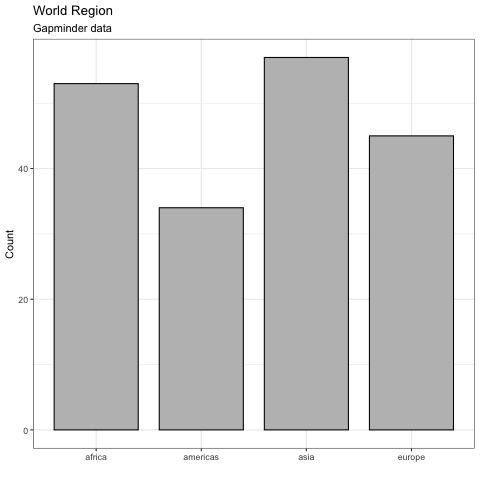
\includegraphics[width=0.75\textwidth]{images/bar_plot.png}
  \label{fig:barplot}
 \caption{Bar plot. Rappresentazione grafica di una variabile categorica. Ciascuna modalit\`a viene rappresentata da una barra, la cui dimensione \`e proporzionale alla sua frequenza, in questo caso assoluta.}
\end{figure}


\subsection{Relazione tra due variabili categoriche}

La funzione \lsin{table()} pu\`o anche essere usata per costruire \textbf{tabelle di contingenza}:

\begin{lstlisting}[style=Rstylescript]
tab_cont <- table(gapminder$world_region, gapminder$income_group_2017)
\end{lstlisting}

\begin{lstlisting}[style=Rstyle]
tab_cont	
         High income Low income Middle income
africa             1         27            25
americas           8          1            25
asia              15          2            40
europe            30          0            15
\end{lstlisting}
%
Notiamo che, di nuovo, le variabili sono ordinate in ordine alfabetico. La tabella sarebbe per\`o di pi\`u facile interpretazione se le colonne fossero ordinate da low a high income:

\begin{lstlisting}[style=Rstylescript]
ord <- c(2, 3, 1) 
tab_cont <- tab_cont[, ord]
\end{lstlisting}

\begin{lstlisting}[style=Rstyle]
tab_cont
           Low income Middle income High income
  africa           27            25           1
  americas          1            25           8
  asia              2            40          15
  europe            0            15          30
\end{lstlisting}
%
Questa tabella di contingenza mostra le frequenze assolute. Per ottenere le frequenze relative a partire da quelle assolute usiamo di nuovo la funzione \lsin{prop.table()}:

\begin{lstlisting}[style=Rstylescript]
tab_cont_rel <- prop.table(tab_cont)
\end{lstlisting}
%
senza nessun argomento, ci ritorna la frequenza relativa di ciascuna coppia di modalit\`a nel dataset, e come tale, somma a 1:


\begin{lstlisting}[style=Rstyle]
tab_cont_rel
            Low income Middle income High income
  africa   0.142857143   0.132275132 0.005291005
  americas 0.005291005   0.132275132 0.042328042
  asia     0.010582011   0.211640212 0.079365079
  europe   0.000000000   0.079365079 0.158730159
  
sum(tab_cont_rel)
[1] 1
\end{lstlisting}
%
Per creare le frequenze relative per righe o per colonne, si usa il parametro \lsin{margin}, che prende il valore \lsin{1} per le righe e \lsin{2} per le colonne:

\begin{lstlisting}[style=Rstylescript]
tab_cont_rel_row <- prop.table(tab_cont, margin=1)
tab_cont_rel_col <- prop.table(tab_cont, margin=2)
\end{lstlisting}


\begin{lstlisting}[style=Rstyle]
tab_cont_rel_row
         Low income Middle income High income
africa   0.50943396    0.47169811  0.01886792
americas 0.02941176    0.73529412  0.23529412
asia     0.03508772    0.70175439  0.26315789
europe   0.00000000    0.33333333  0.66666667

tab_cont_rel_col
         Low income Middle income High income
africa   0.90000000    0.23809524  0.01851852
americas 0.03333333    0.23809524  0.14814815
asia     0.06666667    0.38095238  0.27777778
europe   0.00000000    0.14285714  0.55555556
\end{lstlisting}


\vspace{0.5cm} 

\begin{exercise}\label{ex4.2}
	
\noindent Scrivere il codice per trasformare la frequenza relativa contenuta in \lsin{tab_cont_rel_col} in percentuale, con una sola cifra decimale.

\noindent Per ciascuna classe di income, qual \`e la regione del mondo con la frequenza pi\`u alta?

\end{exercise}


\subsection{Mosaic plot}

Le tabelle di contingenza possono essere visualizzate come \textbf{Mosaic plot} usando la funzione \lsin{mosaicplot()}:

\begin{lstlisting}[style=Rstylescript]
mosaicplot(tab_cont)
\end{lstlisting}
%
Possiamo renderlo pi\`u chiaro usando i colori (anche a costo di aggiungere informazione ridondante):

\begin{lstlisting}[style=Rstylescript]
mosaicplot(tab_cont, color = c("darkgreen", "gray70", "darkmagenta"))
\end{lstlisting}
%
e le etichette per assi e titolo, ottenendo il grafico mostrato in Figura~\ref{fig:mosaic}:

\begin{lstlisting}[style=Rstylescript]
mosaicplot(tab_cont, color = c("darkgreen", "gray70", "darkmagenta"), xlab ="World Region", ylab = "Income group", main="Income group by world region")
\end{lstlisting}


\begin{figure}[h]
 \centering
  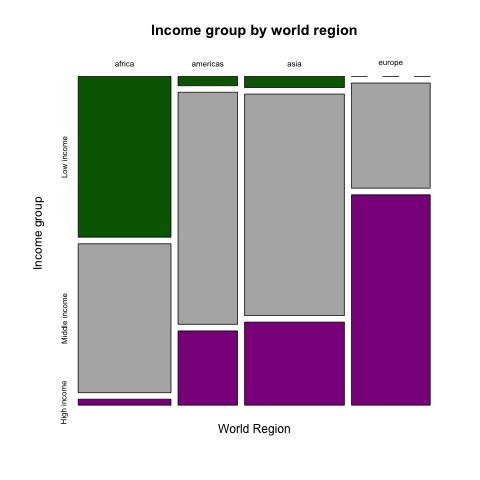
\includegraphics[width=0.75\textwidth]{images/mosaic_plot.png}
  \label{fig:mosaic}
 \caption{Mosaic plot. Rappresentazione grafica della relazione tra due variabili categoriche: world region (sull'asse delle ascisse) e income group (sull'asse delle ordinate). I rettangoli sono colorati in base all'income group, con verde, grigio e viola a indicare alto, medio e basso income, rispettivamente. Ogni rettangolo mostra la percentuale di osservazioni per ciascuna coppia di modalit\`a delle due variabili. La linea tratteggiata indica che non \`e presente nessuna osservazione per l'intersezione di due modalit\`a (paesi europei con low income).}
\end{figure}

\section{I dati numerici}

\subsection{Misure di centralit\`a e dispersione}
\label{sec:centdisp}

R offre delle funzioni per calcolare diverse misure sia di  centralit\`a sia di dispersione. Per la \textbf{media} e la \textbf{deviazione standard} usiamo:

\begin{lstlisting}[style=Rstylescript]
mean_happiness <- mean(gapminder$happiness_score_2011)
sd_happiness <- sd(gapminder$happiness_score_2011)
\end{lstlisting}

\begin{lstlisting}[style=Rstyle]
mean_happiness
[1] NA

sd_happiness
[1] NA
\end{lstlisting}
%
cosa \`e successo? Se ci sono dei valori a \lsin{NA}, R ritorner\`a \lsin{NA}. Come facciamo ad escluderli? Con il parametro \lsin{na.rm}:

\begin{lstlisting}[style=Rstylescript]
mean_happiness <- mean(gapminder$happiness_score_2011, na.rm=TRUE)
sd_happiness <- sd(gapminder$happiness_score_2011, na.rm=TRUE)
\end{lstlisting}

\begin{lstlisting}[style=Rstyle]
mean_happiness
[1] 54.05252

sd_happiness
[1] 10.81201
\end{lstlisting}
%
Calcoliamo ora \textbf{mediana} e \textbf{quartili}, \textbf{massimo} e \textbf{minimo}:

\begin{lstlisting}[style=Rstylescript]
median_happiness <- median(gapminder$happiness_score_2011, na.rm=TRUE)
quartile_happiness <- quantile(gapminder$happiness_score_2011, na.rm=TRUE)

min_happiness <- min(gapminder$happiness_score_2011, na.rm=TRUE)
max_happiness <- max(gapminder$happiness_score_2011, na.rm=TRUE)
\end{lstlisting}

\begin{lstlisting}[style=Rstyle]
median_happiness
[1] 52.3

quartile_happiness
   0%   25%   50%   75%  100%
29.40 46.75 52.30 62.85 77.90

min_happiness
[1] 29.4

max_happiness
[1] 77.9
\end{lstlisting}


\vspace{0.5cm} 

\begin{exercise}\label{ex4.3}
	
\noindent Scrivere il codice per calcolare range e range interquartile.

\noindent Secondo voi, alla luce di tutte le statistiche calcolate, che forma ha questa distribuzione?

\end{exercise}

\subsection{Istogrammi}
\label{sec:histo}

Andiamo ora a costruirne l'\textbf{istogramma}, di nuovo passo passo:

\begin{lstlisting}[style=Rstylescript]
ggplot(gapminder, aes(x=happiness_score_2011)) + geom_histogram()
\end{lstlisting}

\begin{lstlisting}[style=Rstyle]
`stat_bin()` using `bins = 30`. Pick better value
with `binwidth`.
(*@\textbf{\textcolor{red}{Warning message: }}@*)
Removed 50 rows containing non-finite outside the
scale range (`stat_bin()`).
\end{lstlisting}
%
questo messaggio ci sta dando numerose informazioni: \emph{(i)} \lsin{ggplot} sta creando 30 gruppi (bins, corrispondenti a 30 barre), andando a dividere i vostri dati equamente in questi bins e \emph{(ii)} 50 righe del vostro dataset sono state eliminate perch\`e non hanno un valore finito. Cosa possono essere questi valori non finiti? 

\noindent Se avete risposto \lsin{NA}, avete ragione. Andiamo a verificarlo:

\begin{lstlisting}[style=Rstyle]
is.na(gapminder$happiness_score_2011)
  [1] FALSE FALSE FALSE  TRUE FALSE  TRUE FALSE FALSE
  [9] FALSE FALSE FALSE  TRUE FALSE FALSE  TRUE FALSE
 [17] FALSE  TRUE FALSE  TRUE FALSE FALSE FALSE FALSE
 [25]  TRUE FALSE FALSE FALSE FALSE FALSE FALSE  TRUE
 [33] FALSE FALSE FALSE FALSE FALSE FALSE FALSE FALSE
 [41] FALSE  TRUE FALSE  TRUE FALSE FALSE FALSE FALSE
 [49]  TRUE FALSE FALSE FALSE FALSE  TRUE  TRUE FALSE
 [57]  TRUE  TRUE FALSE FALSE FALSE  TRUE FALSE FALSE
 [65] FALSE FALSE  TRUE FALSE FALSE  TRUE  TRUE FALSE
 [73] FALSE FALSE FALSE  TRUE FALSE FALSE FALSE FALSE
 [81] FALSE FALSE FALSE FALSE FALSE FALSE FALSE FALSE
 [89]  TRUE FALSE FALSE FALSE FALSE FALSE FALSE  TRUE
 [97]  TRUE FALSE FALSE FALSE FALSE FALSE  TRUE FALSE
[105] FALSE  TRUE FALSE FALSE FALSE  TRUE FALSE  TRUE
[113] FALSE FALSE FALSE FALSE  TRUE  TRUE  TRUE FALSE
[121] FALSE FALSE FALSE FALSE  TRUE  TRUE FALSE FALSE
[129]  TRUE FALSE FALSE  TRUE FALSE FALSE FALSE FALSE
[137] FALSE FALSE FALSE FALSE FALSE  TRUE  TRUE  TRUE
[145] FALSE FALSE FALSE  TRUE FALSE FALSE FALSE FALSE
[153]  TRUE  TRUE FALSE FALSE  TRUE FALSE FALSE  TRUE
[161]  TRUE  TRUE FALSE  TRUE FALSE  TRUE FALSE FALSE
[169] FALSE FALSE FALSE  TRUE FALSE  TRUE FALSE FALSE
[177] FALSE FALSE  TRUE FALSE FALSE FALSE FALSE  TRUE
[185] FALSE FALSE FALSE FALSE FALSE
\end{lstlisting}
%
Se state pensando di contare quanti \lsin{TRUE} ci sono, sappiate che \lsin{TRUE} equivale a \lsin{1} in R, e che \lsin{FALSE} equivale a \lsin{0}. Quindi possiamo sommare tutti i \lsin{TRUE} con la funzione \lsin{sum()}:

\begin{lstlisting}[style=Rstyle]
num_na <- is.na(gapminder$happiness_score_2011)
sum(num_na)
[1] 50
\end{lstlisting}
%
\lsin{ggplot} ha effettivamente scartato i valori a \lsin{NA}.

\noindent Ignoriamo perci\`o questo warning e andiamo ora a lavorare sul numero di bins, usando il parametro \lsin{binwidth}, come suggerito da R, e nel migliorarne la grafica, con gli stessi parametri che abbiamo visto per il bar plot:

\begin{lstlisting}[style=Rstylescript]
ggplot(gapminder, aes(x=happiness_score_2011)) + geom_histogram(binwidth=5, width=0.8, fill="gray", color="black")
\end{lstlisting}
%
Sistemiamo ora labels, titolo e sfondo, ottenendo il grafico in Figura~\ref{fig:histogram} e assegniamolo a una variabile:

\begin{lstlisting}[style=Rstylescript]
histogram_happiness <- ggplot(gapminder, aes(x=happiness_score_2011)) + geom_histogram(binwidth=5, width=0.8, fill="gray", color="black") + xlab("Score") + ylab("Counts") + ggtitle("World happiness in 2011", subtitle="Gapminder data") + theme_bw()
\end{lstlisting}


\begin{figure}[h]
 \centering
  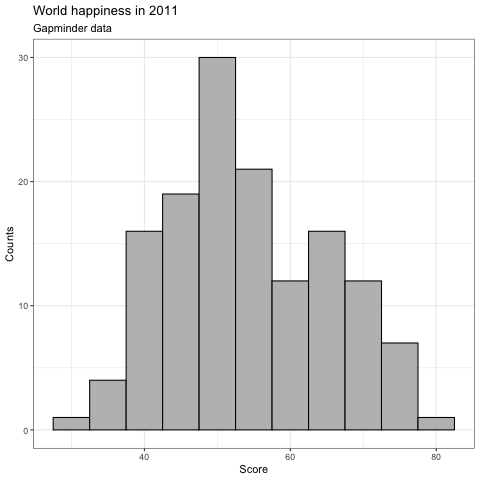
\includegraphics[width=0.75\textwidth]{images/histogram.png}
  \label{fig:histogram}
 \caption{Istogramma. Rappresentazione grafica di una variabile numerica. La variabile subisce un processo di Discretizzazione, che identifica un certo numero di classi, ognuna rappresentata da una barra, la cui dimensione \`e proporzionale alla sua frequenza, in questo caso assoluta.}
\end{figure}

\vspace{0.5cm} 

\begin{exercise}\label{ex4.4}
	
\noindent Scrivere il codice per calcolare tutte le statistiche descritte in precedenza per l'attributo \lsin{gov_health_spending_percent}.

\noindent Costruirne poi l'istogramma, colorando le barre di bianco con dei bordi rossi.

\end{exercise}

\subsubsection{Box plot}
\label{sec:boxplot}

Visualizziamo ora coma si distribuisce il livello di felicit\`a a seconda dell'income group usando un \textbf{boxplot}:

\begin{lstlisting}[style=Rstylescript]
ggplot(gapminder, aes(x=happiness_score_2011, y=income_group_2017)) + geom_boxplot()
\end{lstlisting}

\begin{lstlisting}[style=Rstyle]
(*@\textbf{\textcolor{red}{Warning message: }}@*)
Removed 50 rows containing non-finite outside the
scale range (`stat_boxplot()`).
\end{lstlisting}
%
anche questa volta l'income group viene visualizzato in ordine alfabetico, ma andarne a cambiare l'ordine \`e un po' pi\`u complesso di quello che abbiamo fatto per il mosaic plot. Infatti, \lsin{ggplot2} trasforma i dati categorici in \lsin{factor}, un tipo di dato che non avevamo ancora introdotto. Vediamoli adesso:

\begin{lstlisting}[style=Rstyle]
income_group <- gapminder$income_group_2017

class(income_group)
[1] "character"

income_group <- as.factor(income_group)

class(income_group)
[1] "factor"

head(income_group)
[1] Low income    Middle income Middle income
[4] High income   Middle income High income   
Levels: High income Low income Middle income
\end{lstlisting}
%
quello che vogliamo andare a riordinare sono i livelli:

\begin{lstlisting}[style=Rstylescript]
gapminder$income_group_2017 <- factor(gapminder$income_group_2017, levels=c("Low income", "Middle income", "High income"))	
\end{lstlisting}

\begin{lstlisting}[style=Rstyle]
head(gapminder$income_group_2017)
[1] Low income    Middle income Middle income
[4] High income   Middle income High income  
Levels: Low income Middle income High income
\end{lstlisting}
%
Torniamo quindi al nostro boxplot:

\begin{lstlisting}[style=Rstylescript]
ggplot(gapminder, aes(x=happiness_score_2011, y=income_group_2017)) + geom_boxplot()
\end{lstlisting}
%
I gruppi sono ora ordinati. Miglioriamone ora la grafica, ottenendo il grafico mostrato in Figura~\ref{fig:boxplot}:


\begin{lstlisting}[style=Rstylescript]
boxplot <- ggplot(gapminder, aes(x=happiness_score_2011, y=income_group_2017)) + geom_boxplot(fill="grey") + xlab("Score") + ylab("") + ggtitle("World happiness by income group", subtitle="Gapminder data") + theme_bw()
\end{lstlisting}

\begin{figure}[h]
 \centering
  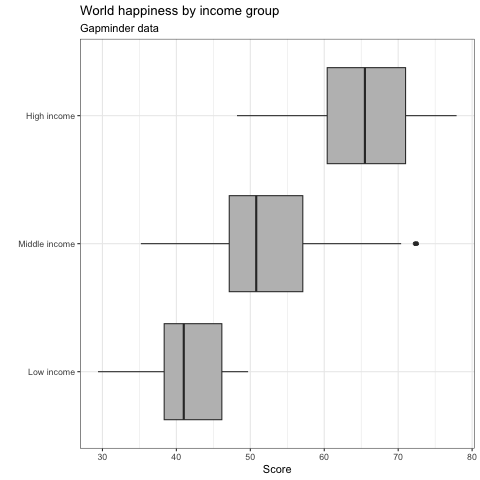
\includegraphics[width=0.75\textwidth]{images/boxplot.png}
  \label{fig:boxplot}
 \caption{Boxplot. Rappresentazione grafica congiunta di una variabile numerica e una variabile categorica. La variabile numerica viene rappresentata utilizzando, in questo caso, tre diversi boxplot, uno per ciascuna variabile categorica. Questo ci permette di confrontare le tre distribuzioni.}
\end{figure}


\vspace{0.5cm} 

\begin{exercise}\label{ex4.5}
	
\noindent Scrivere il codice per costruire il boxplot che mostra le differenze in happiness score a seconda delle world region.

\noindent In quale regione le persone sono meno felici? \\

\noindent \textbf{Difficolt\`a elevata:} Qual \`e l'happiness score medio in ogni regione? 


	\exnote{Suggerimenti}%
	\begin{myitemize}
		\item Per calcolare l'happiness score medio, dovete estrarre solo la porzione di dati che appartiene a una data regione.
	\end{myitemize}

\end{exercise}


\section{La relazione tra due variabili numeriche}

Andiamo ora a utilizzare il \textbf{coefficiente di Pearson} per calcolare la \textbf{correlazione} tra happiness score e health spending:

\begin{lstlisting}[style=Rstylescript]
cr <- cor(x=gapminder$gov_health_spending_percent, y=gapminder$happiness_score_2011)
\end{lstlisting}

\begin{lstlisting}[style=Rstyle]
[1] NA
\end{lstlisting}
%
Abbiamo di nuovo il problema con gli \lsin{NA}, usiamo il manuale per risolverlo:

\begin{lstlisting}[style=Rstyle]
?cor
\end{lstlisting}

\begin{lstlisting}[style=Rstylescript]
cr <- cor(x=gapminder$gov_health_spending_percent, y=gapminder$happiness_score_2011, use="complete.obs")
\end{lstlisting}

\begin{lstlisting}[style=Rstyle]
[1] 0.3985756
\end{lstlisting}

\subsection{Scatter plot}

\begin{figure}[h]
 \centering
  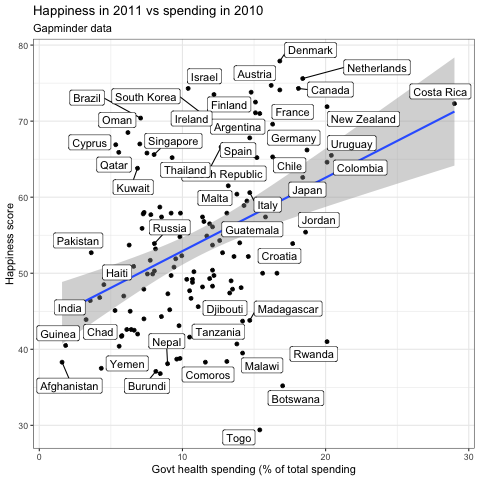
\includegraphics[width=0.75\textwidth]{images/scatter.png}
  \label{fig:scatter}
 \caption{Scatter plot. Rappresentazione grafica della relazione tra due variabili numeriche. Ciascun asse mostra una delle due variabili, la linea di tendenza (in blu) viene mostrata insieme al suo intervallo di confidenza.}
\end{figure}

Visualizziamo ora la relazione tra l'happiness score e lo spending percentage usando uno \textbf{scatterplot}:

\begin{lstlisting}[style=Rstylescript]
ggplot(gapminder, aes(x=gov_health_spending_percent, y=happiness_score_2011)) + geom_point() 
\end{lstlisting}

\begin{lstlisting}[style=Rstyle]
(*@\textbf{\textcolor{red}{Warning message: }}@*)
Removed 57 rows containing missing values or values outside the scale range (`geom_point()`).
\end{lstlisting}
%
Perch\'e ora ci sono 57 valori a \lsin{NA}?

\begin{lstlisting}[style=Rstylescript]
scatter <- ggplot(gapminder, aes(x=gov_health_spending_percent, y=happiness_score_2011)) + geom_point() + xlab("Govt health spending (% of total spending") + ylab("Happiness score") + ggtitle("Happiness in 2011 vs spending in 2010", subtitle="Gapminder data") + theme_bw()
\end{lstlisting}
%
Andiamo per ultimo ad aggiungere una linea di tendenza:

\begin{lstlisting}[style=Rstylescript]
scatter <- scatter + geom_smooth(method="lm")
\end{lstlisting}
%
Possiamo anche mettere un'etichetta per mostrare alcuni dei paesi, come mostrato in Figura~\ref{fig:scatter}, usando il pacchetto R \lsin{ggrepel} (che avete installato durante l'Esercizio 2.5, Sezione~\ref{sec:R_package}):

\begin{lstlisting}[style=Rstylescript]
library(ggrepel)
scatter <- scatter + geom_label_repel(aes(label = country)
\end{lstlisting}




\vspace{0.5cm}

\begin{tcolorbox}[width=1\linewidth, halign=left, colframe=blue!60, colback=white, boxsep=1mm, arc=3mm]

\textbf{Punti principali}

\begin{myitemize}
    \item Usare \lsin{nrow(), ncol(), dim(), colnames(), head()} e \lsin{tail()} per esplorare la struttura di un data frame 
    \item Usare \lsin{table()} e \lsin{prop.table()} per calcolare frequenze assolute e relative
	\item Usare \lsin{mean(), sd(), median(), quantile(), min()} e \lsin{max()} per calcolare le corrispondenti misure di centralit\`a e dispersione
    \item Usare la funzione \lsin{is.na()} e il parametro \lsin{na.rm} per gestire i valori a \lsin{NA}
    \item Usare \lsin{cor} per calcolare la correlazione tra due variabili numeriche
    \item Usare il pacchetto R \lsin{ggplot2} per visualizzare i dati
\end{myitemize}

\end{tcolorbox}

\chapter{La statistica inferenziale}
\label{cap:inferenziale}

\section*{Obiettivi di apprendimento}


\begin{multicols}{2}
\begin{tcolorbox}[width=1\linewidth, halign=left, colframe=blue!60, colback=white, boxsep=1mm, arc=3mm]

Domande

\begin{myitemize}
	\item Quali funzioni R offre per rappresentare una distribuzione Normale?
	\item Come posso calcolare un intervallo di confidenza?
	\item Come posso eseguire un test di ipotesi per la differenza di medie o di proporzioni?
\end{myitemize}

\end{tcolorbox} 
\columnbreak
\begin{tcolorbox}[width=1\linewidth, halign=left, colframe=blue!60, colback=white, boxsep=1mm, arc=3mm]

Obiettivi

\begin{myitemize}
	\item Saper calcolare la probabilit\`a di un'osservazione sapendo che si distribuisce secondo una Normale
	\item Saper calcolare un intervallo di confidenza
	\item Saper eseguire test di ipotesi per la differenza di medie e proporzioni
\end{myitemize}

\end{tcolorbox} 
\columnbreak
\end{multicols}


\section{La distribuzione Normale}

R offre una famiglia di funzioni per simulare e gestire una distribuzione Normale, di cui vedremo solo due:

\begin{myitemize}
	\item \lsin{pnorm(q, mean = 0, sd = 1, lower.tail = TRUE)}:  calcola l’area relativa (ricordiamo che l’area totale \`e sempre uguale a 1) sotto la curva dal valore dato di \lsin{q} fino a meno infinito (se \lsin{lower.tail = TRUE}) o pi\`u infinito (se \lsin{lower.tail = FALSE})
	\item \lsin{qnorm(p, mean = 0, sd = 1, lower.tail = TRUE)}: \`e l'inversa (opposta) di \lsin{pnorm} e ci ritorna il valore per cui l'area relativa  calcolata da meno infinito (se \lsin{lower.tail = TRUE}) o da pi\`u infinito (se \lsin{lower.tail = FALSE}) vale \lsin{p}.
\end{myitemize}
%
e che quindi possono essere usate come classiche tavole delle distribuzioni\footnote{Come quelle che abbiamo visto a lezione.}. 

\vspace{0.5cm} 

\begin{exercise}\label{ex5.1}

\noindent Che tipo di distribuzione Normale \`e quella assunta come default dalle funzioni che abbiamo appena elencato? \\

\noindent Che valori restituiscono i seguenti comandi?

\begin{lstlisting}[style=Rstyle]
pnorm(0, mean = 0, sd = 1, lower.tail = TRUE)
pnorm(0, mean = 0, sd = 1, lower.tail = FALSE)

pnorm(1.96, mean=0, sd = 1, lower.tail = TRUE)
pnorm(1.96, mean=0, sd = 1, lower.tail = FALSE)

pnorm(-1.96, mean=0, sd = 1, lower.tail = TRUE)

qnorm(0.5, lower.tail = TRUE)
qnorm(0.025, lower.tail = FALSE)
\end{lstlisting}

\end{exercise}


\vspace{0.5cm} 

\begin{exercise}\label{ex5.2}

\noindent Il peso alla nascita dei gemelli inglesi si distribuisce secondo una distribuisce Normale con media $2404 \text{ g}$ e deviazione standard $580 \text{ g}$. 

\begin{myitemize}
	\item Qual \`e la probabilit\`a che un gemello pesi meno di $1500 \text{ g}$?
	\item Qual \`e la proporzione di gemelli che pesano meno di $1500 \text{ g}$?
\end{myitemize}

\end{exercise}

\section{Intervalli di confidenza}
\label{sec:CI}

Per calcolare l'intervallo di confidenza (CI), dobbiamo ricordare che la sua formula \`e:

$$
\text{CI} = stima \pm \text{valore critico} \times \text{standard error}.
$$

\noindent dove la quantit\`a $\text{valore critico} \times \text{standard error}$ \`e il margine di errore.


\noindent Andiamo quindi a calcolare il 95\% CI per una media, sapendo che $\text{SE} = \frac{\sigma}{\sqrt{n}}$.
%
Supponiamo che in un campione di 760 uomini inglesi riporti di avere avuto in media $\bar{x} = 11.4$ partner eterosessuali, con una deviazione standard di $11.2$. Il primo passo \`e calcolare lo standard error:


\begin{lstlisting}[style=Rstylescript]
n <- 760
x <- 11.4
sd <- 11.2

se <- sd/sqrt(n)
\end{lstlisting}

\begin{lstlisting}[style=Rstyle]
se
[1] 0.4062667
\end{lstlisting}
%
che useremo poi per calcolarci il margine di errore. Prima di calcolare il margine di errore, ci serve per\`o sapere qual \`e il valore critico, ovvero lo $z$-score che corrisponde a un'area del $100-95=5\%$, ovvero a un'area di $0.05/2$ per ciascuna coda:

\begin{lstlisting}[style=Rstylescript]
v <- qnorm(0.025, lower.tail = FALSE)
\end{lstlisting}

\begin{lstlisting}[style=Rstyle]
v
[1] 1.959964
\end{lstlisting}

\begin{lstlisting}[style=Rstylescript]
me <- v * se
\end{lstlisting}

\begin{lstlisting}[style=Rstyle]
me
[1] 0.7962681
\end{lstlisting}
%
ora possiamo quindi calcolare il margine superiore e inferiore del nostro CI:

\begin{lstlisting}[style=Rstylescript]
lCI <- x - me
uCI <- x + me
\end{lstlisting}

\begin{lstlisting}[style=Rstyle]
lCI
[1] 10.60373
uCI
[1] 12.19627
\end{lstlisting}
%
andiamo ad arrotondarli:

\begin{lstlisting}[style=Rstylescript]
lCI <- round(lCI, 1)
uCI <- round(uCI, 1)
\end{lstlisting}

\begin{lstlisting}[style=Rstyle]
lCI
[1] 10.6
uCI
[1] 12.2
\end{lstlisting}
%
Il 95\% CI \`e quindi compreso tra \lsin{10.6} e \lsin{12.2}.

\vspace{0.5cm} 

\begin{exercise}\label{ex5.3}

\noindent Calcolare il 90\% e il 99\% CI per l'esempio precedente.\\

\noindent Quale CI \`e pi\`u largo? Cosa vuol dire?

\end{exercise}


\section{La distribuzione $t$ di Student}

R offre due funzioni \lsin{pt()} e \lsin{qt()} per le distribuzioni $t$ di Student che sono analoghe \lsin{pnorm()} e \lsin{qnorm()}, dove l'unico parametro da specificare sono i gradi di libert\`a (o \emph{degree of freedom}, \lsin{df}):

\noindent Supponiamo di avere un piccolo campione di 15 uomini inglesi che riporti di avere avuto in media $\bar{x} = 11.4$ partner eterosessuali, con una deviazione standard di $11.2$. Il primo passo \`e calcolare lo standard error, che si calcola come in precedenza:


\begin{lstlisting}[style=Rstylescript]
n <- 15
x <- 11.4
sd <- 11.2

se <- sd/sqrt(n)
\end{lstlisting}

\begin{lstlisting}[style=Rstyle]
se
[1] 2.891828
\end{lstlisting}
%
quello che cambia \`e il valore critico, ovvero il $t$-score che corrisponde a un'area del $100-95=5\%$, ovvero a un'area di $0.05/2$ per ciascuna coda, in una distribuzione $t$ con $n-1$ gradi di libert\`a:

\begin{lstlisting}[style=Rstylescript]
v <- qt(0.025, df=n-1, lower.tail = FALSE)
\end{lstlisting}

\begin{lstlisting}[style=Rstyle]
v
[1] 2.144787
\end{lstlisting}

\begin{lstlisting}[style=Rstylescript]
me <- v * se
\end{lstlisting}

\begin{lstlisting}[style=Rstyle]
me
[1] 6.202353
\end{lstlisting}
%
ora possiamo quindi calcolare il margine superiore e inferiore del nostro CI:

\begin{lstlisting}[style=Rstylescript]
lCI <- round(x - me, 1)
uCI <- round(x + me, 1)
\end{lstlisting}

\begin{lstlisting}[style=Rstyle]
lCI
[1] 5.2
uCI
[1] 17.6
\end{lstlisting}
%
Per verificare che per campioni grandi il $t$-score converga allo $z$-score andiamo a calcolarlo per \lsin{n=760}, la numerosit\`a campionaria dell'esempio precedente e andiamo a confrontarlo con il corrispondente $z$-score:


\begin{lstlisting}[style=Rstyle]
z <- qnorm(0.025, lower.tail = FALSE)
t <- qt(0.025, df=760-1, lower.tail = FALSE)
\end{lstlisting}

\begin{lstlisting}[style=Rstyle]
z
[1] 1.959964
t
[1] 1.963094

abs(z-t)
[1] 0.003130427
\end{lstlisting}


\section{$t$-test}

Per testare la differenza tra le medie di due distribuzioni\footnote{Stiamo quindi parlando di due variabili continue} si pu\`o usare la funzione \lsin{t.test)}. Essa rappresenta una buona approssimazione dello $z$-test per campioni grandi (come abbiamo appena visto) ed \`e robusta nel caso di campioni piccoli.

\noindent Andiamo quindi a formulare la nostra domanda di ricerca: 

\vspace{0.2cm}

\centerline{\emph{Ci sono differenze in happiness score tra low e high income groups?}} 

\vspace{0.2cm}

\noindent a cui corrisponde la seguente ipotesi nulla: 

\vspace{0.2cm}

\noindent $\mathcal{H}_0$: Non ci sono differenze in happiness score tra low e high income groups.

\vspace{0.2cm}

\noindent Andiamo quindi a estrarre solo i valori relativi a questi due income groups:

\begin{lstlisting}[style=Rstylescript]
gapminder_low_high <- gapminder[gapminder$income_group_2017 != "Middle income", ]
\end{lstlisting}
%
e andiamo a calcolare il $t$-test per un test a due code\footnote{\lsin{t.test()} ci permette di calcolare il test a una coda usando \lsin{less} o \lsin{greater} per l'opzione \lsin{alternative}}. La funzione \lsin{t.test()} pu\`o prendere come input sia due vettori, che rappresentano le distribuzioni empiriche delle variabili da testare, sia una formula (vedi box). 


\begin{mybox}{Formule}

In R, una formula \`e definita come $y ~ x + z$, dove $y$ \`e una variabile dipendente che dipende, appunto, da una o pi\`u variabili indipendenti, $x$ e $z$ nel nostro esempio. \`E un oggetto ricorrente, specialmente quando dobbiamo definire dei modelli. 

\end{mybox}


\noindent Usiamo la versione che richiede una formula:

\begin{lstlisting}[style=Rstylescript]
r <- t.test(happiness_score_2011 ~ income_group_2017, data=gapminder_low_high, alternative = "two.sided")
\end{lstlisting}
%
Se ne visualizziamo l'output possiamo avere molte informazioni:

\begin{lstlisting}[style=Rstyle]
r 

	Welch Two Sample t-test

data:  happiness_score_2011 by income_group_2017
t = -13.777, df = 60.869, p-value < 2.2e-16
alternative hypothesis: true difference in means between group Low income and group High income is not equal to 0
95 percent confidence interval:
 -25.75036 -19.22270
sample estimates:
 mean in group Low income mean in group High income 
                 42.16957                  64.65610 
				 
class(r)	
[1] "htest"

attributes(r)
$names
 [1] "statistic"   "parameter"   "p.value"     "conf.int"   
 [5] "estimate"    "null.value"  "stderr"      "alternative"
 [9] "method"      "data.name"  

$class
[1] "htest"

r$p.value
[1] 2.276535e-20

r$stderr
[1] 1.632151		 
\end{lstlisting}
%
Quindi possiamo rifiutare l'ipotesi nulla con una soglia critica $\alpha = 0.05$, e concludere che esista una differenza in happiness score tra low e high income groups.


\vspace{0.5cm} 

\begin{exercise}\label{ex5.4}

\noindent Rispondere alla seguente domanda di ricerca: 

\centerline{Ci sono differenze in happiness score tra Europa e le Americhe?}

\end{exercise}

\section{Mann-Whitney test}

\noindent Supponiamo ora di aver formulato la seguente domanda di ricerca: 

\vspace{0.2cm}

\centerline{\emph{Ci sono differenze in spesa sanitaria tra Asia e Africa?}}

\vspace{0.2cm}

\noindent a cui corrisponde la seguente ipotesi nulla:

\vspace{0.2cm}

\noindent $\mathcal{H}_0$: Non ci sono differenze in spesa sanitaria tra Asia e Africa

\vspace{0.2cm}

\noindent Supponiamo anche di non volere/potere fare nessuna assunzione sulle Normalit\`a delle distribuzioni di queste variabili. Quello che possiamo usare \`e il Mann-Whitney test che può essere utilizzato in tutti quei casi in cui non \`e possibile e/o consigliabile effettuare un confronto tra medie\footnote{\`E un test non parametrico.}. Attenzione che questo test si esegue, in R, con la funzione \lsin{wilcox.test()}, che abbiamo visto essere il test che si usa per il confronto in campioni appaiati\footnote{\`E un altro test non parametrico.}. R usa la stessa funzione per il Mann-Whitney e il Wilcoxon test e li distingue grazie a un parametro, \lsin{paired}, che \`e a \lsin{FALSE} per il primo test e a \lsin{TRUE} per il secondo quando si passa in input due vettori. Quando si passa in input una formula, R assume che si voglia effettuare il Mann-Whitney test\footnote{Come la funzione \lsin{t.test()}, anche \lsin{wilcox.test()} accetta due tipi di output.}.

\noindent Andiamo di nuovo a estrarre solo i valori relativi a questi due continenti:

\begin{lstlisting}[style=Rstylescript]
gapminder_africa_asia <- gapminder[gapminder$world_region %in% c("asia", "africa"), ]
\end{lstlisting}
%
e andiamo a calcolare il test a due code\footnote{\lsin{wilcox.test()} ci permette di calcolare il test a una coda usando \lsin{less} o \lsin{greater} per l'opzione \lsin{alternative}}, Andiamo anche a richiedere il calcolo dell'intervallo di confidenza\footnote{Il comportamento di default \`e di non calcolarlo} e lo andiamo a fissare al 95\%:

\begin{lstlisting}[style=Rstylescript]
rw <- wilcox.test(gov_health_spending_percent ~ world_region, data=gapminder_africa_asia, alternative = "two.sided", conf.int=TRUE, conf.level=0.95)
\end{lstlisting}

\begin{lstlisting}[style=Rstyle]
rw 

	Wilcoxon rank sum test with continuity
	correction

data:  gov_health_spending_percent by world_region
W = 1376, p-value = 0.8682
alternative hypothesis: true location shift is not equal to 0
95 percent confidence interval:
 -1.640034  1.830045
sample estimates:
difference in location 
             0.1599579 
\end{lstlisting}
%
Quindi non possiamo rifiutare l'ipotesi nulla con una soglia critica $\alpha = 0.05$, e concludere che esista una differenza in spesa sanitaria tra Asia e Africa.



\section{$\chi^2$ test}

Andiamo ora ad applicare il processo di \textbf{discretizzazione} alla nostra variabile continua happiness score per ottenere due gruppi di (circa) uguale dimensione, uno dei quali rappresenter\`a il gruppo con uno score di felicit\`a alta e uno quello di felicit\`a bassa. 

\noindent Quale statistica divide esattamente a met\`a i miei dati?

\begin{lstlisting}[style=Rstylescript]
gapminder$happiness_group <- ifelse(gapminder$happiness_score_2011 < median_happiness, "low", "high")

#Calcoliamnone la frequenza assoluta
happiness_group <- table(gapminder$happiness_group)
\end{lstlisting}


\begin{lstlisting}[style=Rstyle]
happiness_group

high  low 
  70   69
\end{lstlisting}

\vspace{0.5cm} 

\begin{exercise}\label{ex5.5}

\noindent Discretizzare lo spending governativo in due gruppi di (circa) uguale dimensione, uno dei quali rappresenter\`a il gruppo di paesi che spendono molto in sanit\`a e uno quello che spendono poco 

\end{exercise}

\noindent Supponiamo ora di aver formulato la seguente domanda di ricerca: 

\vspace{0.2cm}

\centerline{\emph{Ci sono differenze tra paesi che hanno una spesa sanitaria}}
\centerline{\emph{alta o bassa a e avere una felicit\`a alta o bassa?}}

\vspace{0.2cm}

\noindent a cui corrisponde la seguente ipotesi nulla:

\vspace{0.2cm}

\noindent $\mathcal{H}_0$: Non ci sono differenze tra paesi che hanno una spesa sanitaria alta o bassa e avere una felicit\`a alta o bassa

\vspace{0.2cm}

\noindent Quello che vogliamo fare \`e andare a testare se ci sono differenze nelle proporzioni di queste due variabili categoriche\footnote{Sono diventate categoriche grazie al processo di discretizzazione che abbiamo appena applicato.}. Andiamo quindi ad applicare il $\chi^2$ test, iniziando con il crearci la tabella di contingenza delle due variabili:

\begin{lstlisting}[style=Rstylescript]
tab_spending_happiness <- table(gapminder$happiness_group, gapminder$spending_group)
\end{lstlisting}

\begin{lstlisting}[style=Rstyle]
tab_spending_happiness 
       
        low  high
  low    43    23
  high   25    41

prop.table(tab_spending_happiness )
       
              low      high
  low   0.3257576 0.1742424
  high  0.1893939 0.3106061
\end{lstlisting}
%
e andiamo a calcolare il $\chi^2$:

\begin{lstlisting}[style=Rstylescript]
rp <- chisq.test(tab_spending_happiness)
\end{lstlisting}
%
di nuovo, se ne visualizziamo l'output possiamo avere molte informazioni:

\begin{lstlisting}[style=Rstyle]
rp

Pearson's Chi-squared test with Yates' continuity correction

data:  tab_spending_happiness
X-squared = 8.7656, df = 1, p-value = 0.00307	 
\end{lstlisting}
%
Quindi possiamo rifiutare l'ipotesi nulla con una soglia critica $\alpha = 0.05$, e concludere che ci sono differenze tra paesi che hanno una spesa sanitaria alta o bassa e avere una felicit\`a alta o bassa.


\section{Fisher's exact test}


\noindent Supponiamo ora di aver formulato la seguente domanda di ricerca: 

\vspace{0.2cm}

\centerline{\emph{Ci sono differenze tra income groups e avere una felicit\`a alta o bassa?}}

\vspace{0.2cm}

\noindent a cui corrisponde la seguente ipotesi nulla:

\vspace{0.2cm}

\noindent $\mathcal{H}_0$: Non ci sono differenze tra income groups e avere una felicit\`a alta o bassa

\vspace{0.2cm}

\noindent Andiamo quindi a crearci la tabella di contingenza delle due variabili in oggetto:

\begin{lstlisting}[style=Rstylescript]
tab_income_happiness <- table(gapminder$income_group_2017, gapminder$happiness_group)
\end{lstlisting}

\begin{lstlisting}[style=Rstyle]
tab_income_happiness 
       
                low  high
  Low income     23     0
  Middle income  42    33
  High income     4    37
\end{lstlisting}
%
Notiamo che ci sono due caselle con frequenze assolute $< 5$, il $\chi^2$ ci \`e quindi precluso e dobbiamo usare invece il Fisher's test:

\begin{lstlisting}[style=Rstylescript]
rf <- fisher.test(tab_income_happiness)
\end{lstlisting}
%

\begin{lstlisting}[style=Rstyle]
rf

	Fisher's Exact Test for Count Data

data:  tab_income_happiness
p-value = 6.014e-14
alternative hypothesis: two.sided				 
\end{lstlisting}
%
Quindi possiamo rifiutare l'ipotesi nulla con una soglia critica $\alpha = 0.05$ e concludere che ci sono differenze tra income groups e avere una felicit\`a alta o bassa.


\vspace{0.5cm} 

\begin{exercise}\label{ex5.6}

\noindent Rispondere alla seguente domanda di ricerca: 

\centerline{\emph{Ci sono differenze tra world regions e avere una felicit\`a alta o bassa?}}

	\exnote{Suggerimenti}%
	\begin{myitemize}
		\item Visualizzate la tabella di contingenza per decidere quale sia il test da usare.
	\end{myitemize}

\end{exercise}








\vspace{0.5cm}

\begin{tcolorbox}[width=1\linewidth, halign=left, colframe=blue!60, colback=white, boxsep=1mm, arc=3mm]

\textbf{Punti principali}

\begin{myitemize}
    \item Usare \lsin{pnorm()} per calcolare l'area relativa sottesa a una curva Normale e \lsin{qnorm()} per fare l'operazione inversa
    \item Usare \lsin{pt()} per calcolare l'area relativa sottesa a una curva $t$ di Student e \lsin{qt()} per fare l'operazione inversa
	\item Usare \lsin{t.test} per eseguire un test di ipotesi per la differenza di medie (test parametrico)
	\item Usare \lsin{wilcox.test()} per eseguire un test di ipotesi casi in cui non \`e possibile/consigliabile effettuare un confronto tra medie (test non-parametrico)
    \item Usare \lsin{chisq.test} e \lsin{fisher.test} per eseguire un test di ipotesi per la differenza di proporzioni 
\end{myitemize}

\end{tcolorbox}



\appendix
\chapter{Soluzioni agli esercizi}

\section{Capitolo 3}

\begin{solution}{ex2.1}

\noindent I seguenti nomi di variabile sono validi in R:

\begin{lstlisting}[style=Rstyle]
min_height
max.height
MaxLength
celsius2kelvin
\end{lstlisting}

\noindent anche questo nome \`e valido, la sua particolarit\`a \`e che Crea una variabile nascosta:

\begin{lstlisting}[style=Rstyle]
.mass
\end{lstlisting}

\noindent mentre i seguenti nomi di variabile non sono validi:

\begin{lstlisting}[style=Rstyle]
_age
min-length
2widths
\end{lstlisting}


\end{solution}

\vspace{0.5cm}

\begin{solution}{ex2.2}

\begin{lstlisting}[style=Rstyle]
# Assegna a mass il valore 50.5
x <- 50.5    

# Assegna a age il valore 122
y <- 122     

# Moltiplica il valore contenuto in x per 2 e lo ri-assegna 
x <- x * 2   

# Sottrae 20 al valore contenuto in y e lo ri-assegna 
y <- y - 20  
	
x
[1] 101
y
[1] 102
\end{lstlisting}

\end{solution}

\vspace{0.5cm}

\begin{solution}{ex2.3}

\noindent Due dei comandi che possono essere usati sono:

\begin{lstlisting}[style=Rstyle]
x > y	
[1] FALSE

x >= y
[1] FALSE
\end{lstlisting}

\end{solution}

\vspace{0.5cm}

\begin{solution}{ex2.4}

\begin{lstlisting}[style=Rstyle]
# Crea la variabile mass e le assegna il valore 2.2
mass <- 2.2   

# Crea la variabile age e le assegna il valore 15
age <- 15     

# Per verificare che esistano posso visualizzare 
# tutte le variabili nell'ambiente di lavoro
ls()
[1] "age" "mass"

# Per verificare che siano state inizializzate correttamente 
# posso stamparle a video 
mass 
[1] 2.2
age 
[1] 15

#Rimuove le due variabili
rm(mass, age)  

# Per verificare che siano state rimosse posso visualizzare 
# tutte le variabili nell'ambiente di lavoro
ls()
character(0)
\end{lstlisting}

\end{solution}


\vspace{0.5cm}

\begin{solution}{ex2.5}

\begin{lstlisting}[style=Rstyle]
# Carico un pacchetto R specificato nella sessione di lavoro
library(ggplot2) 
\end{lstlisting}


\begin{lstlisting}[style=Rstyle]
# Installo il pacchetto specificato (attenzione alle virgolette)
install.packages("ggrepel")  
\end{lstlisting}	

\end{solution}	


\newpage

\section{Capitolo 4}

\begin{solution}{ex3.1}

\begin{lstlisting}[style=Rstyle]
df$country
 [1] "Benin"      "Greece"     "Tanzania"  
 [4] "Estonia"    "Russia"     "Syria"     
 [7] "Zambia"     "Vietnam"    "Liberia"   
[10] "Mozambique"
\end{lstlisting}

\noindent Ritorna la prima colonna di un data frame, usandone il nome, come un vettore di caratteri (tipo: \lsin{character}) ed \`e equivalente a:

\begin{lstlisting}[style=Rstyle]
df[, 1]
 [1] "Benin"      "Greece"     "Tanzania"  
 [4] "Estonia"    "Russia"     "Syria"     
 [7] "Zambia"     "Vietnam"    "Liberia"   
[10] "Mozambique"
\end{lstlisting}
%
che usa l'indice di posizione della colonna. Analogamente,

\begin{lstlisting}[style=Rstyle]
df[1, ]
  country world_region income_group_2017
1   Benin       africa        Low income
  happiness_score_2011 gov_health_spending_percent
1                 38.7                         9.6
\end{lstlisting}
%
ritorna non la prima colonna, ma la prima riga. Invece

\begin{lstlisting}[style=Rstyle]
df[1, 1]
[1] "Benin"
\end{lstlisting}
%
ritorna il contenuto della cella in posizione \lsin{<1,1>}.

\begin{lstlisting}[style=Rstyle]
df["country"]
      country
1       Benin
2      Greece
3    Tanzania
4     Estonia
5      Russia
6       Syria
7      Zambia
8     Vietnam
9     Liberia
\end{lstlisting}
%
invece crea un nuovo data frame, andando a tagliare una "fetta" di quello originale.

\end{solution}

\vspace{0.5cm}

\begin{solution}{ex3.2}

\begin{lstlisting}[style=Rstyle]
str(cats)
'data.frame' : 4 obs. of  4 variables:
 $ coat      : chr  "calico" "black" "tabby" "white"
 $ weight    : chr  "2.1" "5" "3.2" "3.3"
 $ playful   : chr  "1" "0" "1" "1"
 $ age       : chr  "2" "3" "5" "9"
\end{lstlisting}
%
Tutte le colonne sono state trasformate in \lsin{character}. Questo \`e successo perch\'e un vettore pu\`o includere un solo tipo di dati, e il meno restrittivo \`e  \lsin{character}.

\end{solution}

\vspace{0.5cm}

\begin{solution}{ex3.3}

\noindent Punto 1: Creare un data frame chiamato \lsin{classe} che contenga le seguenti informazioni su noi stessi: \lsin{<Nome, Cognome, Giorno di Nascita>}

\begin{lstlisting}[style=Rstyle]
classe <- data.frame(Nome = "Alessia",
                     Cognome = "Visconti",
                     GiornoNascita  = 4)
\end{lstlisting}
%
Soluzione alternativa:

\begin{lstlisting}[style=Rstyle]
classe <- data.frame(Nome = c("Alessia"),
                     Cognome = c("Visconti"),
                     GiornoNascita  = c(4))
\end{lstlisting}

\vspace{0.2cm}
\noindent Punto 2: Aggiungere delle righe che contengano le stesse informazioni per due dei vicini:

\begin{lstlisting}[style=Rstyle]
vicino1 <- list("Tizio", "Caio", "12")
vicino2 <- list("Pinco", "Pallino", "20")
classe <- rbind(classe, vicino1)
classe <- rbind(classe, vicino2)
\end{lstlisting}
%
Soluzione alternativa:

\begin{lstlisting}[style=Rstyle]
vicino1 <- list("Tizio", "Caio", "12")
vicino2 <- list("Pinco", "Pallino", "20")
classe <- rbind(classe, vicino1, vicino2)
\end{lstlisting}
%
Soluzione alternativa:

\begin{lstlisting}[style=Rstyle]
classe <- rbind(classe, list("Tizio", "Caio", "12"),
                        list("Pinco", "Pallino", "20"))
\end{lstlisting}
%
Soluzione alternativa:

\begin{lstlisting}[style=Rstyle]
vicini <- data.frame(Nome = c("Tizio", "Pinco"),
                     Cognome = c("Caio", "Pallino"),
                     GiornoNascita  = c(12, 20))
classe <- rbind(classe, vicini))
\end{lstlisting}
%
Altre soluzioni sono possibili.

\vspace{0.2cm}
\noindent Punto 3:  Aggiungere una colonna con la mostra risposta (\lsin{TRUE/FALSE}) alla domanda \emph{Mi servirebbe una pausa?}

\begin{lstlisting}[style=Rstyle]
risposta <- c("FALSE", "TRUE", "FALSE")
classe <- cbind(classe, risposta)
\end{lstlisting}
%
Soluzione alternativa:
\begin{lstlisting}[style=Rstyle]
classe <- cbind(classe, risposta=c("FALSE", "TRUE", "FALSE"))
\end{lstlisting}
%
Altre soluzioni sono possibili.

\end{solution}

\vspace{0.5cm}

\begin{solution}{ex3.4}

\noindent Comando 1:
\begin{lstlisting}[style=Rstyle]
x[2:4]
  b   c   d
6.2 7.1 4.8
\end{lstlisting}
%
\noindent Comando 2:
\begin{lstlisting}[style=Rstyle]
x[-c(1,5)]
  b   c   d
6.2 7.1 4.8
\end{lstlisting}
%
\noindent Comando 3:
\begin{lstlisting}[style=Rstyle]
x[c(2,3,4)]
  b   c   d
6.2 7.1 4.8
\end{lstlisting}

\end{solution}

\vspace{0.5cm}

\begin{solution}{ex3.5}

\begin{lstlisting}[style=Rstyle]
x[4 < x & x < 7]

  a   b   d
5.4 6.2 4.8 
\end{lstlisting}

\end{solution}

\vspace{0.5cm}

\begin{solution}{ex3.6}

\noindent Punto 1: estrarre tutti i valori per paesi europei

\begin{lstlisting}[style=Rstyle]
df[df$world_region == "europe", ]

  country world_region income_group_2017
2  Greece       europe       High income
4 Estonia       europe       High income
5  Russia       europe     Middle income
  happiness_score_2011 gov_health_spending_percent
2                 53.7                       12.10
4                 54.9                       11.70
5                 53.9                        8.04
\end{lstlisting}
%
\noindent Punto 2: estrarre tutti i valori per i paesi non nel gruppo "Middle income"

\begin{lstlisting}[style=Rstyle]
df[df$income_group_2017 != "Middle income", ]
      country world_region income_group_2017
1       Benin       africa        Low income
2      Greece       europe       High income
3    Tanzania       africa        Low income
4     Estonia       europe       High income
9     Liberia       africa        Low income
10 Mozambique       africa        Low income
   happiness_score_2011 gov_health_spending_percent
1                  38.7                         9.6
2                  53.7                        12.1
3                  40.7                        13.8
4                  54.9                        11.7
9                    NA                        11.1
10                 49.7                        12.2
\end{lstlisting}
%
Soluzione alternativa:

\begin{lstlisting}[style=Rstyle]
df[df$income_group_2017 %in% c("High income", "Low income"), ]
\end{lstlisting}
%
\noindent Punto 3: estrarre tutti i valori nella prima, seconda e ultima colonna

\begin{lstlisting}[style=Rstyle]
df[, c(1:2, 5)]
      country world_region gov_health_spending_percent
1       Benin       africa                        9.60
2      Greece       europe                       12.10
3    Tanzania       africa                       13.80
4     Estonia       europe                       11.70
5      Russia       europe                        8.04
6       Syria         asia                        5.58
7      Zambia       africa                       15.60
8     Vietnam         asia                        7.79
9     Liberia       africa                       11.10
10 Mozambique       africa                       12.20
\end{lstlisting}
%
Soluzione alternativa:

\begin{lstlisting}[style=Rstyle]
df[, c(1, 2, 5)]
\end{lstlisting}
%
\noindent Punto 4: estrarre tutti i valori tranne quelli dell'ultima colonna

\begin{lstlisting}[style=Rstyle]
df[, -5]
      country world_region income_group_2017
1       Benin       africa        Low income
2      Greece       europe       High income
3    Tanzania       africa        Low income
4     Estonia       europe       High income
5      Russia       europe     Middle income
6       Syria         asia     Middle income
7      Zambia       africa     Middle income
8     Vietnam         asia     Middle income
9     Liberia       africa        Low income
10 Mozambique       africa        Low income
   happiness_score_2011
1                  38.7
2                  53.7
3                  40.7
4                  54.9
5                  53.9
6                  40.4
7                  50.0
8                  57.7
9                    NA
10                 49.7
\end{lstlisting}
%
Soluzione alternativa:

\begin{lstlisting}[style=Rstyle]
df[, 1:4]
\end{lstlisting}
%
\noindent Punto 5: estrarre la prima, quarta, e quinta colonna per tutti i paesi africani

\begin{lstlisting}[style=Rstyle]
df[df$world_region == "africa", c(1,4,5)]	
      country happiness_score_2011
1       Benin                 38.7
3    Tanzania                 40.7
7      Zambia                 50.0
9     Liberia                   NA
10 Mozambique                 49.7
   gov_health_spending_percent
1                          9.6
3                         13.8
7                         15.6
9                         11.1
10                        12.2	
\end{lstlisting}

\end{solution}

\section{Capitolo 5}


\begin{solution}{ex4.1}

\begin{lstlisting}[style=Rstylescript]
# Calcolo la frequenza assoluta
freq_a_income <- table(gapminder$income_group_2017)

# Calcolo la frequenza relativa, 
freq_r_income <- prop.table(freq_a_income)

# Calcolo le percentuali moltiplicando per 100
freq_r_income <- freq_r_income*100

# Arrotondo a una cifra decimale
freq_r_income <- round(freq_r_income, 1)
\end{lstlisting}

\noindent La moda \`e: "Middle income"

\end{solution}

\vspace{0.5cm}

\begin{solution}{ex4.2}
	
\begin{lstlisting}[style=Rstylescript]
# Calcolo le percentuali moltiplicando per 100
tab_cont_rel_col_percent <- tab_cont_rel_col*100

# Arrotondo a una cifra decimale
tab_cont_rel_col_percent <- round(tab_cont_rel_col_percent, 1)
\end{lstlisting}

\noindent Le regioni al mondo pi\`u frequenti per low, middle e high income sono Africa, Asia e Europa, rispettivamente.

\end{solution}

\vspace{0.5cm}

\begin{solution}{ex4.3}
	
\begin{lstlisting}[style=Rstylescript]
#Calcolo il range come valore massimo meno valore minimo
range_happiness <- max_happiness - min_happiness

#Calcolo IQR come terzo quartile (in posizione 4 del vettore) - primo quartile (in posizione 2)
iqr_happiness <- quartile_happiness[4] - quartile_happiness[2]
\end{lstlisting}

\noindent Potrebbe avere una distribuzione asimmetrica a destra, ma non possiamo sapere se sia bi- o multi-modale.

\end{solution}

\vspace{0.5cm}

\begin{solution}{ex4.4}
	
\begin{lstlisting}[style=Rstylescript]
mean_spending <- mean(gapminder$gov_health_spending_percent)
sd_spending <- sd(gapminder$gov_health_spending_percent)

median_spending <- median(gapminder$gov_health_spending_percent, na.rm=TRUE)
quartile_spending <- quantile(gapminder$gov_health_spending_percent, na.rm=TRUE)

min_spending <- min(gapminder$gov_health_spending_percent, na.rm=TRUE)
max_spending <- max(gapminder$gov_health_spending_percent, na.rm=TRUE)

range_spending <- max_spending - min_spending
iqr_spending <- quartile_spending[4] - quartile_spending[2]

histogram_spending <- ggplot(gapminder, aes(x=gov_health_spending_percent)) + geom_histogram(binwidth=5, width=0.8, fill="white", color="red") + xlab("Score") + ylab("Counts") + ggtitle("Govt health spending in 2010 (% of total spending)", subtitle="Gapminder data") + theme_bw()
\end{lstlisting}

\noindent Per una spiegazione della soluzione di rimanda al testo delle Sezioni~\ref{sec:centdisp} e~\ref{sec:histo}

\end{solution}


\vspace{0.5cm}


\begin{solution}{ex4.5}

\begin{lstlisting}[style=Rstylescript]
boxplot_world_region <- ggplot(gapminder, aes(x=happiness_score_2011, y=world_region)) + geom_boxplot(fill="grey") + xlab("Score") + ylab("") + ggtitle("World happiness by world_region", subtitle="Gapminder data") + theme_bw()
\end{lstlisting}

\noindent Le persone sono meno felici in Africa.

\noindent Per una spiegazione della soluzione di rimanda al testo della Sezione~\ref{sec:boxplot}.

\vspace{0.2cm} 

\noindent Per risolvere l'ultimo punto, bisognava ricordarsi come estrarre parte di un data frame usando dei vettori (e quindi delle operazioni) logici, come introdotto in Sezione~\ref{sec:subsetting}.

\begin{lstlisting}[style=Rstylescript]
happiness_africa <- gapminder$happiness_score_2011[gapminder$world_region == "africa"]
mean(happiness_africa, na.rm=TRUE)

happiness_asia <- gapminder$happiness_score_2011[gapminder$world_region == "asia"]
mean(happiness_asia, na.rm=TRUE)

happiness_europe <- gapminder$happiness_score_2011[gapminder$world_region == "europe"]
mean(happiness_europe, na.rm=TRUE)

happiness_americas <- gapminder$happiness_score_2011[gapminder$world_region == "americas"]
mean(happiness_americas, na.rm=TRUE)
\end{lstlisting}


\end{solution}	

\newpage

\section{Capitolo 6}

\begin{solution}{ex5.1}

\noindent Le funzioni che abbiamo visto assumono come default una normale standardizzata.

\noindent Per rispondere alle domande, bisogna ricordare le propriet\`a della normale, in generale, e della normale standardizzata, in particolare.

\noindent La mediana (che corrisponde alla media, che nella normale standardizzata \`e zero) divide la curva in due parti identiche. Dato che l'area sottesa \`e sempre \lsin{1}, allora l'area a sinistra della mediana (\lsin{lower.tail = TRUE}) e alla sua destra (\lsin{lower.tail = FALSE}) sono entrambe \lsin{0.5}:

\begin{lstlisting}[style=Rstyle]
pnorm(0, mean = 0, sd = 1, lower.tail = TRUE)
[1] 0.5

pnorm(0, mean = 0, sd = 1, lower.tail = FALSE)
[1] 0.5
\end{lstlisting}
%
di conseguenza, il valore per cui si ottiene un'area uguale a \lsin{0.5} per una normale standardizzata \`e zero:

\begin{lstlisting}[style=Rstyle]
qnorm(0.5, lower.tail = TRUE)
[1] 0
\end{lstlisting}


\noindent Uno $z$-score di \lsin{1.96} \`e un valore particolare, che sappiamo corrisponde a un $\alpha$ di \lsin{0.05}, che viene diviso equamente tra la coda destra (1.96, \lsin{lower.tail = TRUE}) e la coda sinistra (-1.96, \lsin{lower.tail = TRUE}), ognuna delle quali vale quindi \lsin{0.025} (circa). Facendo la differenza, si ottiene l'area per .96, \lsin{lower.tail = FALSE}: \lsin{1-0.025=0.975} (circa):

\begin{lstlisting}[style=Rstyle]
pnorm(1.96, mean=0, sd = 1, lower.tail = TRUE)
[1] 0.9750021
pnorm(1.96, mean=0, sd = 1, lower.tail = FALSE)
[1] 0.0249979
 
pnorm(-1.96, mean=0, sd = 1, lower.tail = TRUE)
[1] 0.0249979
\end{lstlisting}
%
di conseguenza, il valore per cui si ottiene un'area uguale a \lsin{0.024} (coda sinistra) per una normale standardizzata \`e \lsin{-1.96} (circa):

\begin{lstlisting}[style=Rstyle]
qnorm(0.025, lower.tail = TRUE)
[1] -1.959964
\end{lstlisting}



\end{solution}

\vspace{0.5cm}	

\begin{solution}{ex5.2}

\noindent Possiamo usare direttamente la funzione \lsin{pnorm} con i parametri dell'esercizio, ricordandoci che vogliamo quelli che pesano meno di $1500 \text{ g}$, quindi la coda sinistra:

\begin{lstlisting}[style=Rstyle]
pnorm(1500, mean = 2404 , sd = 580, lower.tail = TRUE)
[1] 0.05954309
\end{lstlisting}

\noindent Possiamo anche andare a standardizzare il valore che ci interessa (ottenendo cos\`i lo $z$-score), che usiamo poi in \lsin{pnorm} assumendo che si tratti di una normale standardizzata (quindi con valori di default per media e deviazione standard):

\begin{lstlisting}[style=Rstyle]
zscore <- (1500-2404)/580
pnorm(zscore, lower.tail = TRUE)
[1] 0.05954309
\end{lstlisting}

\noindent Proporzione e probabilit\`a coincidono e sono uguali al $6\%$.

\end{solution}

\vspace{0.5cm}

\begin{solution}{ex5.3}

\noindent Sulla falsariga dell'esempio visto in Sezione~\ref{sec:CI}:

\begin{lstlisting}[style=Rstylescript]
# Stime conosciute
n <- 760
x <- 11.4
sd <- 11.2

# Calcolo lo standard error
se <- sd/sqrt(n)

# Calcolo il valore critico per il 90% CI e il corrispondente margine d'errore
z90 <- (1-0.90)/2
v90 <- qnorm(z90, lower.tail = FALSE)
me90 <- v90 * se

# Calcolo il margine superiore e inferiore:
lCI90 <- x - me90
uCI90 <- x + me90

# Calcolo il valore critico per il 99% CI e il corrispondente margine d'errore
z99 <- (1-0.99)/2
v99 <- qnorm(z99, lower.tail = FALSE)
me99 <- v99 * se

# Calcolo il	margine superiore e inferiore:
lCI99 <- x - me99
uCI99 <- x + me99
\end{lstlisting}


\begin{lstlisting}[style=Rstyle]
# Li visualizzo
lCI90
[1] 10.73175
uCI90
[1] 12.06825
 
lCI99
[1] 10.35353
uCI99
[1] 12.44647
\end{lstlisting}

\noindent L'intervallo di confidenza pi\`u largo \`e quello al 99\%, che ha pi\`u probabilit\`a di includere la vera media $\mu$ della popolazione, ma \`e anche meno preciso.

\end{solution}

\vspace{0.5cm}

\begin{solution}{ex5.4}
	
\noindent Definiamo per prima l'ipotesi nulla

\noindent $\mathcal{H}_0$: Non ci sono differenze in happiness score tra Europa e le Americhe

\begin{lstlisting}[style=Rstylescript]
# Seleziono le aree che mi interessano	
gapminder_eu_am <- gapminder[gapminder$world_region %in% c("europe", "americas"), ]

# Calcolo il $t$-test per un test a due code
r <- t.test(happiness_score_2011 ~ world_region, data=gapminder_eu_am, alternative = "two.sided")
\end{lstlisting}

\begin{lstlisting}[style=Rstyle]
# Visualizzo il P-value
r$p.value	
[1] 0.2485322
\end{lstlisting}
%
Quindi non possiamo rifiutare l'ipotesi nulla con una soglia critica $\alpha = 0.05$. Non abbiamo evidenze sufficienti che ci sia differenza tra Europa e le Americhe in termini di happiness score.
	
\end{solution}	


\vspace{0.5cm}

\begin{solution}{ex5.5}

\begin{lstlisting}[style=Rstylescript]
# Discretizzo
gapminder$spending_group <- ifelse(gapminder$gov_health_spending_percent < median_spending, "low", "high")

# Calcolo frequenza assoluta
spending_group <- table(gapminder$spending_group)
\end{lstlisting}


\begin{lstlisting}[style=Rstyle]
spending_group

high  low 
  91   89 
\end{lstlisting}

\end{solution}


\vspace{0.5cm}

\begin{solution}{ex5.6}
	
\noindent Definiamo per prima l'ipotesi nulla

\noindent $\mathcal{H}_0$: Non ci sono differenze tra world regions e avere una felicit\`a alta o bassa

\begin{lstlisting}[style=Rstylescript]
# Creo la tabella di contingenza	
tab_happiness_region <- table(gapminder$happiness_group, gapminder$world_region)
\end{lstlisting}


\begin{lstlisting}[style=Rstyle]
tab_happiness_region
       
        africa americas asia europe
  low       34        3   20     12
  right      4       19   20     27
\end{lstlisting}

\noindent Ci sono due celle con frequenza assoluta $< 5$, devo quindi usare il Fisher's test:


\begin{lstlisting}[style=Rstylescript]
rf2 <- fisher.test(tab_happiness_region)
\end{lstlisting}

\begin{lstlisting}[style=Rstyle]
# Visualizzo il P-value
rf2$p.value
[1] 9.054219e-10
\end{lstlisting}
%
Rifiutiamo l'ipotesi nulla con una soglia critica $\alpha = 0.05$ e concludiamo che ci siano differenze tra worls region e avere una felicit\`a alta o bassa.
	
\end{solution}	

\end{document}
